\section{MPC regulátor}
Ako už bolo v úvode spomenuté, práca spája viacero odborov do jednej implementácie. Táto časť preto je venovaná návrhu a overenia MPC regulátora.
\subsection{Teoretický základ MPC}
V tejto časti sa vysvetlí história, matematický základ a variácie MPC regulátora.
\subsubsection{On-line MPC}
Prediktívny regulátor je, na najnižšej úrovni, metóda riadenia dynamických systémov, ktorá využíva nástroje matematickej optimalizácie. Spoločné črty všetkých prístupov riešenia problému prediktívnych regulátorov je vypočítať on-line, v každej časovej vzorke,  optimálny riadiaci zásah v konečnom horizonte predikcie pre dynamický model systému, kde aktuálny stav je počiatočný stav. Iba prvý element z vypočítanej sekvencie predikovaných riadiacich zásahov je potom aplikovaný na systém. V ďalšom okamihu vzorkovania je horizont predikcie posunutý a výpočet optimálneho riadiaceho zásahu je vykonávaný znovu pre novonadobudnutý stav. Táto myšlienka nie je nová, už v článku od Lee a Markus (1967), je možné nájsť nasledujúce tvrdenie: ,,Jedna technika na návrh regulátora so spätnou väzbou zo znalosti regulátora pre otvorenú slučku je merať aktuálny stav riadenia procesu a veľmi rýchlo vypočítať funkciu riadenia pre otvorenú slučku. Prvá časť tejto funkcie je potom využitá počas krátkeho intervalu, po ktorom je opäť zmeraný stav procesu a k nemu vypočítaná riadiaca funkcia pre otvorenú slučku. Táto procedúra je potom opakovaná.`` Technika popisovaná v článku od Lee a Markus (1967) je zvyčajne označovaná ako ,,Receding Horizon Control`` (RHC) – ,,Postupujúci horizont riadenia`` a dnes je viac-menej používaný ako synonymum k pojmu,,Model Predictive Control`` – ,,Prediktívne riadenie``. \cite{MPC03} Popisovaný princíp je znázornený na obrázku \ref{01_rec_horizon}.
\begin{figure}[h]
\centering
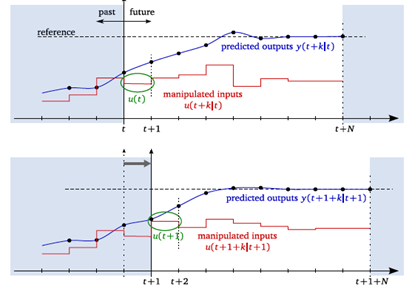
\includegraphics[width=0.75\textwidth]{01_rec_horizon.png}
\caption{Postupujúci horizont riadenia}
\label{01_rec_horizon}
\end{figure}
Nech existuje lineárny dynamický model s časovo invariantnými parametrami, vyjadrený diskrétnou stavovou rovnicou:
\begin{equation} \label{eq1}
\begin{split}
x(t+1)=Ax(t)+Bu(t), \\
y(t)=Cx(t)+Du(t), \\
x(t)∈R^n, y(t)∈R^P, u(t)∈R^m, \\
A∈R^{(n×n)}, B∈R^{(n×m)}, C∈R^{(p×n)}
\end{split}
\end{equation}
x, y, u sú stavy systému, výstupy systému a riadiace zásahy v uvedenom poradí v čase alebo lepšie povedané vo vzorke t. \\
n – predstavuje počet stavov systému \\
p – predstavuje počet výstupov \\
m – predstavuje počet vstupov \\
Matice A, B, C sú systémová matica, vstupná matica a výstupná matica v uvedenom poradí. System \ref{eq1} musí spĺňať nasledujúce obmedzenia na stav a vstup:
\begin{equation} \label{eq2}
\begin{split}
x(t)∈X,u(t)∈U \\
U⊂R^m \\
X⊂R^n
\end{split}
\end{equation}
kde obmedzujúca množina riadiacich zásahov U je konvexná, kompaktná (uzavretá a ohraničená) a obmedzujúca množina stavov X je konvexná a uzavretá. Pre obidve množiny U a X sa predpokladá, že obsahujú počiatok v ich vnútri.\cite{MPC04}
Najskôr je jednoduchšie vyriešiť optimálne riadenie bez obmedzení. Pozornosť bude upriamená na nájdenie takej optimálnej postupností $u^*$(k), ..., $u^*$(k+N – 1), ktorá bude minimalizovať zvolené kvadratické kritérium a zároveň rešpektovať dynamiku systému. Čo inými slovami znamená, že tento regulátor sa bude snažiť minimalizovať stav a rovnako riadiaci zásah, ešte lepšie povedané ich kvadrát. Ak by teda nebola špecifikovaná referenčná hodnota, ktorú má výstup regulátora sledovať, tak implicitne výstupná veličina prediktívneho regulátora konverguje k hodnote 0 alebo pri systémoch s viacerými výstupmi k nulovému vektoru.\\
N – predstavuje horizont predikcie. Ak je teda systém v stave $x_0$, ktorý poznáme a horizont predikcie je 3, tak do optimalizačnej funkcie vstupujú premenné $x_1$, $x_2$, $x_3$ a $u_1$, $u_2$, $u_3$ kde $u_1$ zabezpečí prechod do stavu $x_1$, $u_2$ do stavu $x_2$ atď. každá premenná x je odvoditeľná z predošlého stavu a prvý stav $x_0$ je známy. Preto jedinou ,,neznámou`` ostáva sekvencia riadiacich zásahov. Jedna z otázok by mohla byť, prečo sa využíva kvadratické kritérium. Ako odpoveď je možné použiť príklad kvality riadenia. Pri hodnotení kvality riadenia sa používajú integrálne kritéria. Existuje jednoduché kritérium, ktoré spraví integrál pod krivkou regulačnej odchýlky. Nevýhodou tohto je, že ak dochádza k preregulovaniu a regulačná odchýlka je záporná, veľkosť plochy je zmenšovaná o tie časti, ktoré sú záporné. Toto sa rieši absolútnym integrálnym kritériom, ktoré spraví zo zápornej regulačnej odchýlky kladnú a teda plocha pod krivkou sa zväčšuje aj pri preregulovaní. Navyše existuje kvadratické kritérium, ktoré okrem toho, že odstraňuje problém so zápornou regulačnou odchýlkou navyše viac penalizuje hodnoty odchýlky väčšie ako 1. Inými slovami, ak je hodnota viac ako 1 o to horšiu kvalitu regulácie bude toto kritérium indikovať. Problém so zápornou regulačnou odchýlkou je znázornený na obrázkoch \ref{02_reg_odch}, \ref{03_reg_odch} a \ref{04_reg_odch}.
\begin{figure}[h]
\centering
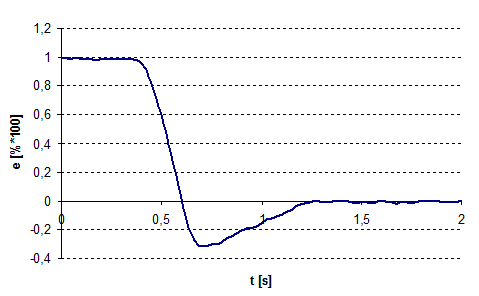
\includegraphics[width=0.90\textwidth]{02_reg_odch.png}
\caption{Hodnota regulačnej odchýlky v čase}
\label{02_reg_odch}
\end{figure}

\begin{figure}[h]
\centering
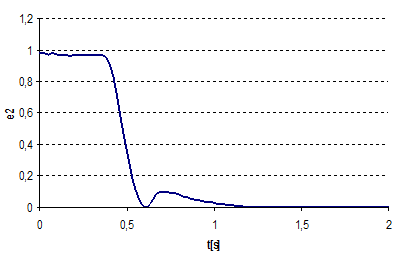
\includegraphics[width=0.90\textwidth]{03_reg_odch.png}
\caption{Časová závislosť kvadrátu regulačnej odchýlky}
\label{03_reg_odch}
\end{figure}
\begin{figure}[h]
\centering
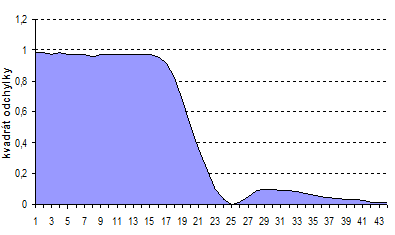
\includegraphics[width=0.90\textwidth]{04_reg_odch.png}
\caption{Plocha kvadrátu regulačnej odchýlky}
\label{04_reg_odch}
\end{figure}

Rovnako ako pri minimalizácii regulačnej odchýlky, tak aj pri minimalizácii riadiaceho zásahu je kvadratické kritérium najlepším ukazovateľom. \\
Pre porozumenie ďalších vzťahov si je potrebné uvedomiť, že: $x(t+k) =x_{(t+k)}$ \\
\begin{itemize}
\item Pre vzorku k = 0 (aktuálny stav systému): x(t)= $x_t$, 
\item pre vzorku k = 1 x(t+1)=$x_{(t+1)}$, 
\item atď.
\end{itemize}
Kvadratické kritérium pre konečný horizont predikcie dĺžky N je:
\begin{equation} \label{eq3}
\begin{split}
J(x(t),u(t),…,u(N-1))=\frac{1}{2}∑_{k=0}^{N-1}[x_k^T Qx_k+u_k^T Ru_k ] +  \frac{1}{2} x_N^T Q_N x_N
\end{split}
\end{equation}
kde:
\begin{equation} \label{eq4}
\begin{split}
x_(k+1)=Ax_k+Bu_k \\
x_0=x(t), \\
Q=Q^T  \succcurlyeq 0,Q_N=Q_N^T \succcurlyeq 0,R=R^T \succ 0 \\
Q_N∈R^{n×n} \\
R∈R^{m×m}
\end{split}
\end{equation}
Matice, Q, $Q_N$ a R sú nazývané váhové matice a spolu s horizontom predikcie N sú nazývané parametrami na ladenie prediktívneho regulátora. Nájdenie optimálneho riadenia, ktoré by minimalizovalo kvadratické kritérium predstavuje dynamickú optimalizáciu a má v tomto prípade aj analytické riešenie: \cite{MPC05}

\begin{equation} \label{eq5}
\begin{split}
x_{t+k}= A^k x_0+ ∑_{i=0}^{k-1}A^i Bu_{k-1-i}\\
u_{t,N}=[u_t^T,…,u_{t+N-1}^T  ]
\end{split}
\end{equation}

Vyjadrenie predikovaného stavu je potom:
\begin{equation} \label{eq6}
\begin{split}
[ x_{t+1}^T,…,x_{t+N}^T  ]^T=Vx_0+Tu_{t,N}
\end{split}
\end{equation}

Táto rovnica je jedna z najdôležitejších pri pochopení fungovania on-line prediktívneho algoritmu. Preto je vhodné ukázať ako matica V a T vyzerajú pre konkrétny jednoduchý systém s horizontom predikcie N = 3 zadaný v stavovom priestore:

\begin{equation} \label{eq7}
\begin{split}
A = \begin{bmatrix}
1 & 0 \\
1 & 1 \\
\end{bmatrix}, 
B = \begin{bmatrix}
0 \\
0,5 \\
\end{bmatrix} \\
C = \begin{bmatrix}
0 & 1 \\
\end{bmatrix}, D = 0 \\
x_{0} = \begin{bmatrix}
4 \\
5 \\
\end{bmatrix} = \begin{bmatrix}
x_{01} \\
x_{02} \\
\end{bmatrix}
\end{split}
\end{equation}
Matice V~a~T budú vyzerať:
\begin{equation} \label{eq8}
\begin{split}
V = \begin{bmatrix}
\begin{matrix}
1 & 0 \\
1 & 1 \\
\end{matrix} \\
\begin{matrix}
1 & 0 \\
2 & 1 \\
\end{matrix} \\
\begin{matrix}
1 & 0 \\
3 & 1 \\
\end{matrix} \\
\end{bmatrix} = \begin{bmatrix}
A^{1} \\
A^{2} \\
A^{3} \\
\end{bmatrix} \\
T = \begin{bmatrix}
\begin{matrix}
1 & 0 & 0 \\
0,5 & 0 & 0 \\
\end{matrix} \\
\begin{matrix}
1 & 1 & 0 \\
1,5 & 0,5 & 0 \\
\end{matrix} \\
\begin{matrix}
1 & 1 & 1 \\
2,5 & 1,5 & 0,5 \\
\end{matrix} \\
\end{bmatrix} = \begin{bmatrix}
\begin{matrix}
A^{0}B & 0\  & 0 \\
\end{matrix} \\
\begin{matrix}
A^{1}B & A^{0}B & 0 \\
\end{matrix} \\
\begin{matrix}
A^{2}B & A^{1}B & A^{0}B \\
\end{matrix} \\
\end{bmatrix}
\end{split}
\end{equation}

Výsledný vzťah:
\begin{equation} \label{eq9}
\begin{split}
{\lbrack\ \begin{bmatrix}
x_{11} \\
x_{12} \\
\end{bmatrix},\ \begin{bmatrix}
x_{21} \\
x_{22} \\
\end{bmatrix},\begin{bmatrix}
x_{31} \\
x_{32} \\
\end{bmatrix}\rbrack}^{T} = \begin{bmatrix}
A^{1} \\
A^{2} \\
A^{3} \\
\end{bmatrix}\begin{bmatrix}
x_{01} \\
x_{02} \\
\end{bmatrix} + \begin{bmatrix}
\begin{matrix}
A^{0}B & 0\  & 0 \\
\end{matrix} \\
\begin{matrix}
A^{1}B & A^{0}B & 0 \\
\end{matrix} \\
\begin{matrix}
A^{2}B & A^{1}B & A^{0}B \\
\end{matrix} \\
\end{bmatrix}\begin{bmatrix}
u_{1} \\
u_{2} \\
u_{3} \\
\end{bmatrix}
\end{split}
\end{equation}
Dôležitý krok pri hľadaní optimálneho riadenia je zo vzťahu \ref{eq3}
„odstrániť`` sumu. Finálny vzťah vyzerá:
\begin{equation} \label{eq10}
\begin{split}
J\left( x\left( t \right),U_{t} \right) = \ \frac{1}{2}{u_{t,N}}^{T}Hu_{t,N} + x^{T}\left( t \right)FU_{t} + \frac{1}{2}x^{T}\left( t \right)\text{Yx}\left( t \right),
\end{split}
\end{equation}

Matica \(\ H \in R^{(m \bullet N \times m \bullet N)}\) ,
\(F \in R^{(n \times m \bullet N)}\), \(Y \in R^{(n \times n)}\). Ak sa
symbol \(\bigotimes\) označí ako kroneckerovo násobenie matíc a
\(I_{j} \in R^{(j \times j)}\), jednotková matica s~príslušnou
dimenziou, tak platí:

\begin{equation} \label{eq11}
\begin{split}
H = \ T^{T}\tilde{Q}T + \ I_{N}\ \bigotimes\ R,\ \ F = V^{T}\tilde{Q}T,\ \ Y = V^{T}\tilde{Q}V \\
\tilde{Q} = \ \begin{bmatrix}
I_{N - 1}\ \bigotimes\ Q & 0 \\
0 & Q_{N} \\
\end{bmatrix}
\end{split}
\end{equation}

Pre systém zo vzťahu \ref{eq7} a~váhy \(Q = Q_{N} = I_{2},\ R = 0,1\) budú
jednotlivé matice vyzerať:

\begin{equation} \label{eq12}
\begin{split}
H = \ \begin{bmatrix}
11,85 & 6,5 & 2,25 \\
6,5 & 4,6 & 1,75 \\
2,25 & 1,75 & 1,35 \\
\end{bmatrix}, F = \begin{bmatrix}
14 & 7,5 & 2,5 \\
4,5 & 2 & 0,5 \\
\end{bmatrix}, \\
Y = \ \ \begin{bmatrix}
17 & 6 \\
6 & 3 \\
\end{bmatrix}
\end{split}
\end{equation}

Optimálnu riadiacu sekvenciu je možné dostať minimalizáciou kvadratickej
formy \ref{eq10}:

\begin{equation} \label{eq13}
\begin{split}
u_{t,N}^{*}\left( x\left( t \right) \right) = \arg{\min_{u_t,N}{\{ J(x\left( t \right),u_{t,N}\ \}}} = - H^{- 1}F^{T}x(t)
\end{split}
\end{equation}

Optimálna hodnota kritéria je:

\begin{equation} \label{eq14}
\begin{split}
J^{*}\left( x\left( t \right) \right) = \min_{u_t,N}{\{ J(x\left( t \right),u_{t,N}\ \}} = \frac{1}{2}x^{T}(t)(Y - FH^{- 1}F^{T})x(t)
\end{split}
\end{equation}

Na to aby sa zabezpečila spätná väzba, je potrebné v~každom kroku použiť
iba prvú hodnotu zo sekvencie riadiacich zásahov a~potom zmerať stav
a~na základe tej hodnoty znovu vypočítať optimálnu sekvenciu riadiacich
zásahov. Bez merania stavu, by to bola regulácia v~otvorenom regulačnom
obvode. Meranie stavu a~jeho použitie pri výpočte nasledujúceho
riadiaceho zásahu v~každom kroku zabezpečí reguláciu v~uzavretom
regulačnom obvode.

\subsubsection{On-line MPC s obmedzením}

Doteraz sa reguloval systém, v~ktorom nebolo žiadne obmedzenie.
V~realite ich však býva mnoho. Pokiaľ sa pri návrhu regulátora začnú
brať do úvahy rovnice \ref{eq2}, bude ich treba zapracovať do výpočtu. Pri
návrhu prediktívneho regulátora s~obmedzením sa využíva kvadratické
programovanie. Úloha kvadratického programovania je úlohou nelineárneho
programovania, v~ktorej sústava ohraničení je lineárna a~účelová funkcia
je kvadratická. Všeobecná formulácia kvadratickej úlohy je:

\begin{equation} \label{eq15}
\begin{split}
f\left( x \right) = \min_{x}\left\{ x^{T}Hx + F^{T}\text{x\ } \right\} \\
x \in D = \{\operatorname{x|}{\ \ Lx \leq m_{c}},\ x \geq 0\}
\end{split}
\end{equation}

Pre návrh regulátora je premenná, ktorej minimum sa hľadá, sekvencia
riadiacich zásahov \(u_{t,N}^{*}\). Rovnice pre prediktívny regulátor
s~obmedzením následne vyzerajú:

\begin{equation} \label{eq16}
\begin{split}
J\left( x\left( t \right),\ u\left( t \right),\ldots,\ u\left( N - 1 \right) \right) = \frac{1}{2}\sum_{k = 0}^{N - 1}\left\lbrack x_{k}^{T}Qx_{k} + u_{k}^{T}Ru_{k} \right\rbrack + \ \frac{1}{2}x_{N}^{T}Q_{N}x_{N}
\end{split}
\end{equation}

kde:
\begin{equation} \label{eq17}
\begin{split}
x_{k + 1} = Ax_{k} + Bu_{k}, \\
x_{0} = x\left( t \right), \\
E_{c}x_{k} + G_{c}u_{k} \leq m_{c},\ \ k = 1\ldots N \\
Q = Q^{T} \succcurlyeq 0,\ Q_{N} = Q_{N}^{T} \succcurlyeq 0,\ R = R^{T} \succ 0
\end{split}
\end{equation}

Aby bolo možné sústavu rovníc \ref{eq16} a \ref{eq17} zapracovať do kvadratického programovania, previesť do maticového tvaru. Prvá časť rovnice ostáva nezmenená, pridá sa k~nej druhá časť:

\begin{equation} \label{eq18}
\begin{split}
J\left( x\left( t \right),U_{t} \right) = \ \frac{1}{2}{u_{t,N}}^{T}Hu_{t,N} + x^{T}\left( t \right)FU_{t} + \frac{1}{2}x^{T}\left( t \right)\text{Yx}\left( t \right), \\
Gu_{t,N} \leq w + Ex(t)
\end{split}
\end{equation}

Kde matice H, F, Y sú určené rovnako ako vo vzťahu \ref{eq11} a~matice G, E, a
vektor w majú tvar:

\begin{equation} \label{eq19}
\begin{split}
G = \begin{bmatrix}
{- I}_{N} \\
\begin{matrix}
I_{N} \\
 - (I_{N}\bigotimes CT) \\
\end{matrix} \\
\begin{matrix}
(I_{N}\bigotimes CT) \\
 \vdots \\
\end{matrix} \\
\end{bmatrix},\ E = \begin{bmatrix}
0 \\
\begin{matrix}
0 \\
 - (I_{N}\bigotimes CV) \\
\end{matrix} \\
\begin{matrix}
(I_{N}\bigotimes CV) \\
 \vdots \\
\end{matrix} \\
\end{bmatrix},\ w = \begin{bmatrix}
 - (1_{N}\bigotimes u_{\min}) \\
\begin{matrix}
(1_{N}\bigotimes u_{\max}) \\
 - (1_{N}\bigotimes y_{\min}) \\
\end{matrix} \\
\begin{matrix}
(1_{N}\bigotimes y_{\max}) \\
 \vdots \\
\end{matrix} \\
\end{bmatrix}
\end{split}
\end{equation}

V rovnici \ref{eq19} sú znázornené základné systémové obmedzenia. Môže
existovať ďaleko viac. \(1_{N}\) predstavuje jednotkový vektor
o~veľkosti N. Prvé dva riadky matice G, \(G_{1,2} \in R^{N \times N}\),
E, \(E_{1,2} \in R^{N \times n}\) a~vektor W, \(W_{1,2} \in R^{N}\) v
(19) predstavujú obmedzenia vstupu. Druhé dva riadky matice G,
\(G_{3,4} \in R^{N \times N}\), E, \(E_{3,4} \in R^{N \times n}\)
a~vektor W, \(W_{3,4} \in R^{N}\) v \ref{eq19} predstavujú obmedzenia výstupu.
Ďalšie obmedzenia, by museli nadobúdať rovnaké rozmery ako predošlé
riadky príslušných matíc a~vektora.

Ak sa pridajú do systému \ref{eq7} obmedzenia na vstup a~výstup:

\begin{equation} \label{eq20}
\begin{split}
- 1 \leq u\left( t \right) \leq 1,\ \  - 10 \leq y\left( t \right) \leq \ 10
\end{split}
\end{equation}

matice G, E a vektor~w budú vyzerajú:

\begin{equation} \label{eq21}
\begin{split}
G = \begin{bmatrix}
{- I}_{3} \\
I_{3} \\
\begin{matrix}
 - (I_{3}\bigotimes CT) \\
(I_{3}\bigotimes CT) \\
\end{matrix} \\
\end{bmatrix},\ E = \begin{bmatrix}
0 \\
\begin{matrix}
0 \\
 - (I_{3}\bigotimes CV) \\
\end{matrix} \\
\begin{matrix}
(I_{3}\bigotimes CV) \\
 \vdots \\
\end{matrix} \\
\end{bmatrix},\ m_{c} = \begin{bmatrix}
 - (1_{3}\bigotimes u_{\min}) \\
(1_{3}\bigotimes u_{\max}) \\
\begin{matrix}
 - (1_{3}\bigotimes y_{\min}) \\
(1_{3}\bigotimes y_{\max}) \\
\end{matrix} \\
\end{bmatrix}
\end{split}
\end{equation}

\begin{equation} \label{eq22}
\begin{split}
G = \begin{bmatrix}
 - \begin{pmatrix}
1 & 0 & 0 \\
0 & 1 & 0 \\
0 & 0 & 1 \\
\end{pmatrix} \\
\begin{pmatrix}
1 & 0 & 0 \\
0 & 1 & 0 \\
0 & 0 & 1 \\
\end{pmatrix} \\
\begin{matrix}
 - \begin{pmatrix}
0,5 & 0 & 0 \\
1,5 & 0,5 & 0 \\
2,5 & 1,5 & 0,5 \\
\end{pmatrix} \\
\begin{pmatrix}
0,5 & 0 & 0 \\
1,5 & 0,5 & 0 \\
2,5 & 1,5 & 0,5 \\
\end{pmatrix} \\
\end{matrix} \\
\end{bmatrix},\ E = \begin{bmatrix}
 - \begin{pmatrix}
0 & 0 \\
0 & 0 \\
0 & 0 \\
\end{pmatrix} \\
\begin{pmatrix}
0 & 0 \\
0 & 0 \\
0 & 0 \\
\end{pmatrix} \\
\begin{matrix}
 - \begin{pmatrix}
1 & 1 \\
2 & 1 \\
3 & 1 \\
\end{pmatrix} \\
\begin{pmatrix}
1 & 1 \\
2 & 1 \\
3 & 1 \\
\end{pmatrix} \\
\end{matrix} \\
\end{bmatrix},\ w = \begin{bmatrix}
\begin{pmatrix}
1 \\
1 \\
\end{pmatrix} \\
\begin{pmatrix}
1 \\
1 \\
\end{pmatrix} \\
\begin{matrix}
\begin{pmatrix}
10 \\
10 \\
\end{pmatrix} \\
\begin{pmatrix}
10 \\
10 \\
\end{pmatrix} \\
\end{matrix} \\
\end{bmatrix}
\end{split}
\end{equation}

Vznikne sústava lineárnych rovníc, ktoré tvoria obmedzenia pre
kvadratický problém.

\begin{equation} \label{eq23}
\begin{split}
\begin{bmatrix}
 - \begin{pmatrix}
1 & 0 & 0 \\
0 & 1 & 0 \\
0 & 0 & 1 \\
\end{pmatrix} \\
\begin{pmatrix}
1 & 0 & 0 \\
0 & 1 & 0 \\
0 & 0 & 1 \\
\end{pmatrix} \\
\begin{matrix}
 - \begin{pmatrix}
0,5 & 0 & 0 \\
1,5 & 0,5 & 0 \\
2,5 & 1,5 & 0,5 \\
\end{pmatrix} \\
\begin{pmatrix}
0,5 & 0 & 0 \\
1,5 & 0,5 & 0 \\
2,5 & 1,5 & 0,5 \\
\end{pmatrix} \\
\end{matrix} \\
\end{bmatrix}\begin{bmatrix}
u_{1} \\
u_{2} \\
u_{3} \\
\end{bmatrix} \leq \begin{bmatrix}
\begin{pmatrix}
1 \\
1 \\
\end{pmatrix} \\
\begin{pmatrix}
1 \\
1 \\
\end{pmatrix} \\
\begin{matrix}
\begin{pmatrix}
10 \\
10 \\
\end{pmatrix} \\
\begin{pmatrix}
10 \\
10 \\
\end{pmatrix} \\
\end{matrix} \\
\end{bmatrix} + \begin{bmatrix}
 - \begin{pmatrix}
0 & 0 & 0 \\
0 & 0 & 0 \\
0 & 0 & 0 \\
\end{pmatrix} \\
\begin{pmatrix}
0 & 0 & 0 \\
0 & 0 & 0 \\
0 & 0 & 0 \\
\end{pmatrix} \\
\begin{matrix}
 - \begin{pmatrix}
1 & 1 \\
2 & 1 \\
3 & 1 \\
\end{pmatrix} \\
\begin{pmatrix}
1 & 1 \\
2 & 1 \\
3 & 1 \\
\end{pmatrix} \\
\end{matrix} \\
\end{bmatrix}\begin{bmatrix}
x_{01} \\
x_{02} \\
\end{bmatrix}
\end{split}
\end{equation}

Ak sú obmedzenia na systém príliš striktné, môže sa stať, že kvadratický
problém nemá riešenie. Takáto situácia je znázornená na obrázku \ref{05_restric}.

\begin{figure}[h]
\centering
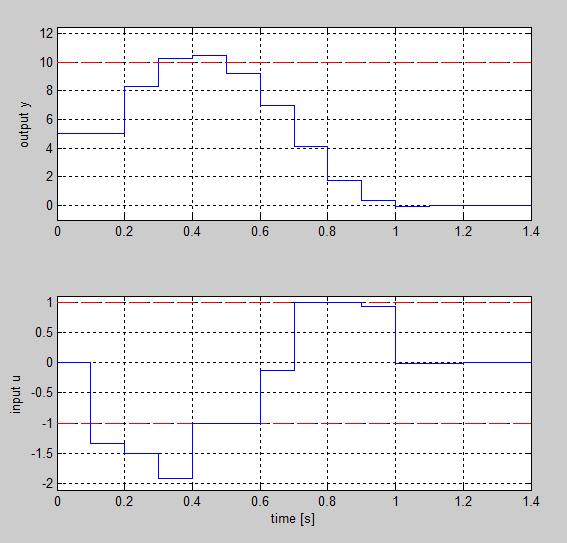
\includegraphics[width=0.99\textwidth]{05_restric.png}
\caption{Časový priebeh výstupnej veličiny a riadiaceho zásahu pre neriešiteľný kvadratický problém. Červená čiara predstavuje obmedzenie na danú veličinu}
\label{05_restric}
\end{figure}

Ak by obmedzenia na výstup boli napríklad
\(- 13 \leq y\left( t \right) \leq \ 13\), kvadratický problém by bol
riešiteľný a~jeho riešenie pre horizont predikcie 3 je zobrazene na
obrázku \ref{06_restric_ok}.

\begin{figure}[h]
\centering
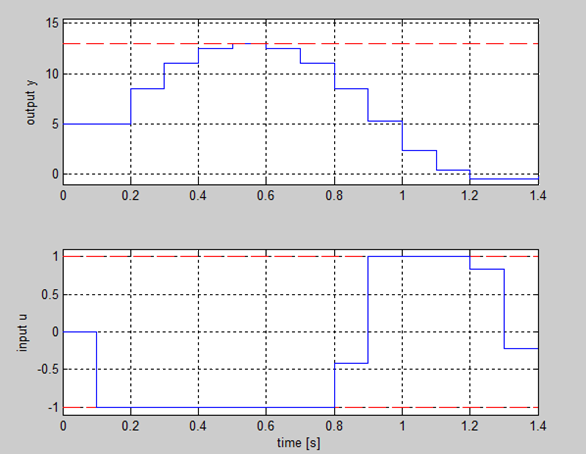
\includegraphics[width=0.99\textwidth]{06_restric_ok.png}
\caption{Časový priebeh výstupnej veličiny a riadiaceho zásahu riešiteľného kvadratického problému}
\label{06_restric_ok}
\end{figure}

\subsubsection{On-line MPC so sledovaním referenčného signálu}
Doteraz bol riešený regulátor, ktorý reguloval hodnotu k „počiatku``
k~hodnote 0 alebo nulovému vektoru. Táto kapitola obsahuje návrh MPC
regulátora, ktorý bude sledovať po častiach konštantný referenčný signál
r(t). Stále sa berie do úvahy systém \ref{eq1}. Najprv je potrebné nahradiť
člen \(x_{k}^{T}Qx_{k}\) v~pôvodnom kritériu \ref{eq17} odchýlkou

\begin{equation} \label{eq24}
\begin{split}
{(z_{k} - r_{k})}^{T}Q_{y}(z_{k} - r_{k})
\end{split}
\end{equation}

kde

\begin{equation} \label{eq25}
\begin{split}
z\left( t \right) = Zy\left( t \right),\ z\left( t \right) \in R^{p_{z}},\ p_{z} \leq p,\ r \leq m
\end{split}
\end{equation}

Aby to bolo možné, je potrebné poznať predikovanú hodnotu referenčného
signálu. Ta môže byť definovaná rôznymi spôsobmi jedna z~možností:
r(t+1)=r(t).

V~ustálenom stave je potrebné, aby platila rovnosť \(z_{u} = r_{u}\).
Takže:

\begin{equation} \label{eq26}
\begin{split}
\begin{bmatrix}
I_{n} - A & - B \\
\text{ZC} & 0 \\
\end{bmatrix}\ \begin{bmatrix}
x_{u} \\
u_{u} \\
\end{bmatrix} = \begin{bmatrix}
0 \\
r_{u} \\
\end{bmatrix}
\end{split}
\end{equation}


Ak ma predchádzajúca matica plnú riadkovú hodnosť, existuje riešenie \(u_{u}\)
a \(x_{u}.\). V~dôsledku nenulového ustáleného vstupu sa v~praxi často
používa odchýlka \(u_{k} = u_{k} - u_{k - 1}\). Ak sústava obsahuje
integrátor, je lepšie použiť hodnotu u. \cite{MPC05}

Kritérium pre sledovanie referencie má tvar:

\begin{equation} \label{eq27}
\begin{split}
J\left( x\left( t \right),\ u\left( t \right),\ldots,\ u\left( N - 1 \right) \right) = \frac{1}{2}\sum_{k = 0}^{N - 1}\left\lbrack e_{k}^{T}Q_{e}e_{k} + u_{k}^{T}Ru_{k} \right\rbrack
\end{split}
\end{equation}

kde 

\begin{equation} \label{eq28}
\begin{split}
e_{k} = y_{k} - r_{k}
\end{split}
\end{equation}

je regulačná odchýlka a

\begin{equation} \label{eq29}
\begin{split}
\Delta u_{k} = u_{k} - u_{k - 1}
\end{split}
\end{equation}

je optimalizovaná premenná. Systém rozšírený o~históriu riadiaceho
zásahu \(u_{k}\) a~generátor referencie \(r_{k}\) je formulovaný:

\begin{equation} \label{eq30}
\begin{split}
\begin{bmatrix}
x_{k + 1} \\
u_{k} \\
r_{k + 1} \\
\end{bmatrix} = \begin{bmatrix}
A & B & 0 \\
0 & I_{m} & 0 \\
0 & 0 & I_{n_{y}} \\
\end{bmatrix}\ \begin{bmatrix}
x_{k} \\
u_{k - 1} \\
r_{k} \\
\end{bmatrix} + \begin{bmatrix}
B \\
I_{m} \\
0 \\
\end{bmatrix}u_{k} = \ A_{m}\hat{x_{k}} + B_{m}u_{k} \\
e_{k} = \begin{bmatrix}
C & 0 & - I_{n_{y}} \\
\end{bmatrix}\hat{x_{k}} = C_{m}\hat{x_{k}}
\end{split}
\end{equation}

\begin{figure}[h]
\centering
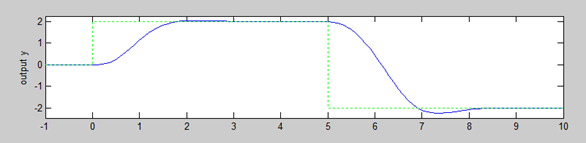
\includegraphics[width=0.99\textwidth]{07_ref.png}
\caption{Sledovanie referencie,  časové priebehy -  zelená referencia, modrá výstup systému}
\label{07_ref}
\end{figure}

Po upravení algoritmu na sledovanie po častiach spojitého referenčného signálu už MPC regulátor neriadi výstupnú veličinu k 0 hodnote alebo vektoru, ale ku aktuálnej hodnote prípadne vektoru referenčného signálu v kroku k, \dots, k + N - 1, kde N predstavuje horizont predikcie. Preto referenčný signál vstupujúci do výpočtu je je buď vektor pre jednorozmerné systémy (SISO) alebo matica pre viacrozmerné systémy (MIMO). Časový priebeh výstupnej veličiny SISO systému regulovaného MPC regulátorom so sledovaním referencie je znázornený na obrázku \ref{07_ref}.

\subsubsection{Explicitné riešenie - offline MPC}

Je zrejmé, že optimálna hodnota kritéria \ref{eq14} a~optimálna riadiaca sekvencia \ref{eq13} (aj s~obmedzeniami) sú funkciou stavu x(t). Túto úlohu je možné formulovať pomocou \textbf{multiparametrického kvadratického
programovania} (mp-QP), ktoré sa snaží nájsť optimálne riešenie pre
všetky možné hodnoty parametra x(t) vopred. Ak sa spraví substitúcia
rovnice

\begin{equation} \label{eq31}
\begin{split}
J^{*}\left( x\left( t \right) \right) = \min_{u_t,N}\left\{ J\left( x\left( t \right),u_{t}) \right|Gu_{t} \leq W + Ex(t) \right\}
\end{split}
\end{equation}

pomocou

\begin{equation} \label{eq32}
\begin{split}
u_{t} = \tilde{u_{t}} - H^{- 1}F^{T}x(t)
\end{split}
\end{equation}

vznikne:

\begin{equation} \label{eq33}
\begin{split}
J^{*}\left( x\left( t \right) \right) = \min_{u_t,N}\left\{ J\left( \tilde{u_{t}},x\left( t \right)) = \frac{1}{2}{\tilde{u}}_{t}^{T}H{\tilde{u}}_{t} + \beta \right|G{\tilde{u}}_{t} \leq W + Sx(t) \right\}
\end{split}
\end{equation}

Kde \(S = E + GH^{- 1}F^{T}\)
a~\(\beta = \frac{1}{2}{x\left( t \right)}^{T}\left( FH^{- 1}F^{T} + Y \right)x(t)\).
Ešte je potrebné zaviesť množinu indexov
I\(= \left\{ 1,\ldots,\ q \right\},\ \)ktorá zodpovedá riadkom matice G,
W a S. \\
Kritický región CR je taká polytopická oblasť v~priestore parametrov
x(t), ktorá má v~optimálnej hodnote
\(J^{*}\left( x\left( t \right) \right),\ u^{*}\left( x\left( t \right) \right)\)
aktívne rovnaké obmedzenia \(A(x(t)) \subset I\). Takže platí

\begin{equation} \label{eq34}
\begin{split}
G_{A}{\tilde{u_{t}}}^{*}\left( x\left( t \right) \right) = W_{A} + S_{A}x\left( t \right)\ pre\ x(t) \in CR
\end{split}
\end{equation}

Nech \(H \succ 0\) a~nech \(G_{A}\)majú lineárne nezávisle riadky, potom
optimálna sekvencia
\({\tilde{u_{t}}}^{*}\left( x\left( t \right) \right)\) je jednoznačne
definovaná afinnou funkciou stavu x(t) na danom kritickom regióne CR.

\begin{equation} \label{eq35}
\begin{split}
{\tilde{u_{t}}}^{*}\left( x\left( t \right) \right) = H^{- 1}G_{A}^{T}(G_{A}H^{- 1}G_{A}^{T})(W_{A} + S_{A}x\left( t \right))
\end{split}
\end{equation}

Ak sa preformuluje optimalizačný problém \ref{eq13} (s obmedzeniami) ako mp-QP
a \(H \succ 0\), potom optimálna riadiaca sekvencia
\({u_{t}}^{*}\left( x\left( t \right) \right):X_{\text{feas}} \rightarrow R^{m}\)
je spojitá, po častiach afinná funkcia na polyedry a~optimálna hodnota
\(J^{*}(x\left( t \right))\) je spojitá, konvexná a~po častiach
kvadratická funkcia na polyedry.

Algoritmus mp-QP najskôr spočíta riešenie (13) (s obmedzeniami) pre
vhodne zvolenú počiatočnú podmienku (\(x_{0} \in X_{\text{feas}}\))
a~vytvorí sa príslušný kritický región CR\textsubscript{0}. Potom
rekurzívne prehľadá okolie a~vytvára nové regióny. Výsledkom je
rozdelenie oblasti \(X_{\text{feas}}\)do kritických regiónov
\(CR_{i} = \left\{ x \right|P_{i}x \leq p_{i}\}\), nad ktorými je
definovaná spojitá afinná funkcia:

\begin{equation} \label{eq36}
\begin{split}
{u_{t}}^{*}\left( x\left( t \right) \right) = F_{i}x\left( t \right) + G_{i}
\end{split}
\end{equation}

a spojitá kvadratická funkcia

\begin{equation} \label{eq37}
\begin{split}
{J_{t}}^{*}\left( x\left( t \right) \right) = x^{T}\left( t \right)A_{i}x\left( t \right) + B_{i}x\left( t \right) + C_{i}
\end{split}
\end{equation}

Týmto sa presunula numerická výpočtová náročnosť optimalizácie \ref{eq13} k~off-line výpočtom. V~priebehu riadenia stačí identifikovať región CR\textsubscript{i}, obsahujúci aktuálny stav x(t) a~aplikovať príslušný
zákon riadenia \label{eq36}. \cite{MPC05} \\
Takýmto spôsobom je možné rozdeliť výpočtovú zložitosť na dve časti. Prvá, výpočtovo zložitejšia, časť je hľadanie kritických regiónov, ktorá sa môže uskutočniť pred zavedením regulátora do behu. Tuto nie je čas kritický, pretože regulačný proces nebeží. Druhá časť je počas behu regulačného procesu. Tá predstavuje časovo nenáročnú operáciu vyhľadania kritického regiónu v pamäti a podľa neho vrátiť akčný zásah. Hlavná nevýhoda offline - explicitného riešenia je, že systém je jednorázovo daný a už počas behu nevstupuje do výpočtu na rozdiel od online riešenia, kde do každého kroku matematický model systému vstupuje a teda je možné  matematický model dynamicky adaptovať, aby čo najviac zodpovedal reálnemu systému. Pri voľbe spôsobu implementácie praktickej časti pre výučbu aj neskôr v IoT prostredí, tento fakt zavážil a zvolila sa online metóda implementácie.
\subsection{Popis funkčnosti On-line MPC algoritmu}
Vytvorený algoritmus sa skladá skladá z viacerých modulov - funkcií naprogramovaných v prostredí Matlab a prispôsobených na fungovanie v open source verzii Octave. Programbol vytvorený pre účely využitia v pedagogickom procese grafické rozhranie bolo vytvorené pomocou komponent Matlabu - Guide, ktorý slúži práve na vytváranie grafických rozhraní. Základné komponenty, z ktorých sa program a  skladá sú znázornené na obrázku \ref{16_com}.
\begin{figure}[h]
\centering
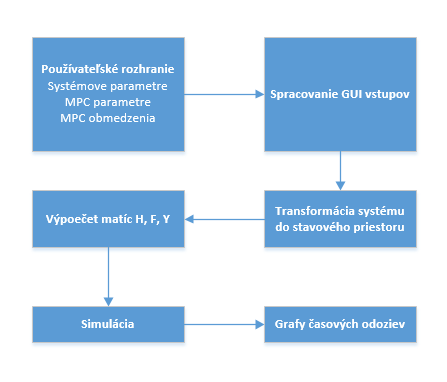
\includegraphics[width=0.8\textwidth]{16_com.png}
\caption{Základné komponenty}
\label{16_com}
\end{figure}

\begin{enumerate}
  \item
    Používateľské rozhranie je popísane v kapitole \ref{mpcprogram}
  \item
    Spracovanie vstupov zabezpečí správnu konverziu reťazcov na čísla a výsledné čísla priradí do správnych premenných potrebných na vstupe do ďalšej časti.
  \item
    MPC regulátor pre svoje fungovanie vždy potrebuje mať na vstupe   matematický model systému podľa rovnice \ref{eq1}, ktorý sa označuje ako systém zadaný v stavovom priestore. Táto časť zabezpečí konverziu z prenosovej funkcie na stavový priestor.
  \item
   Nasleduje výpočet matíc H, F, Y podľa rovníc \ref{eq11}, ktoré sú produktom matíc A, B, C z rovnice \ref{eq1} a váhových matíc, Q, $Q_n$ a R z rovnice \ref{eq11}, ktoré si používateľ volí.
   \item
   Následne prebieha simulácia, ktorej komponenty sú znázornené na obrázku \ref{17_dsim} a popísane nižšie.
   \item
   Produktom simulácie sú dáta, ktoré vytvoria grafy časových odoziev popísaných v kapitole \ref{mpcprogram}.
\end{enumerate}

\begin{figure}[h]
\centering
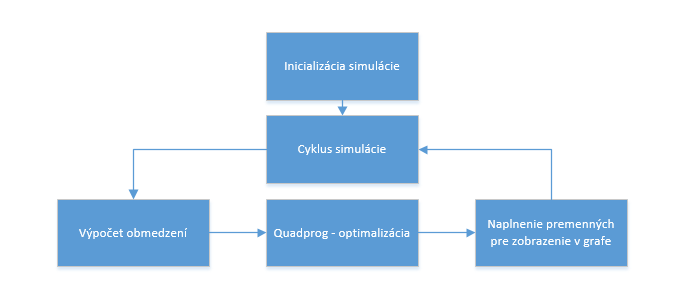
\includegraphics[width=1.1\textwidth]{17_dsim.png}
\caption{Detail komponentu simulácia}
\label{17_dsim}
\end{figure}
\begin{enumerate}
  \item
	Počas inicializácie simulácie sa pripravuje referenčný signál, počiatočný stav systému a počet krokov simulácie.
  \item
    Počet krokov simulácie je nastavený na podiel času simulácie a periódy vzorkovania.
  \item
    V prvej fáze simulačného cyklu sa prepočítajú obmedzenia systému podľa rovnice \ref{eq19}.
  \item 
    Následne prebehne samotná optimalizácia spustením Matlab súčasti \textit{quadprog}, prípade Octave súčasti \textit{qp}. Bez obmedzení by to bol výpočet podľa rovnice \ref{eq13} spomenuté súčasti kvadratického programovania k tomu pridajú sústavu obmedzení.
  \item
    Po optimalizácii sa vyberie prvý akčný zásah z vektora akčných zásahov, ktorý má dĺžku horizontu predikcie, čo je vlastne výsledok optimalizácie. Keďže v programe beží simulačný cyklus tak sa vypočíta výstup, a stav, ktoré sa zapamätajú a následne začína ďalší krok simulačného cyklu.
\end{enumerate}


\subsection{Overenie On-line MPC algoritmu} \label{mpcprogram}
Po teoretickom základe a popise vytvoreného algoritmu nasleduje popis grafického rozhrania a jeho overenie. Grafické rozhranie vytvoreného programu je znázornené na obrázku \ref{08_gui} 

\begin{figure}[h]
\centering
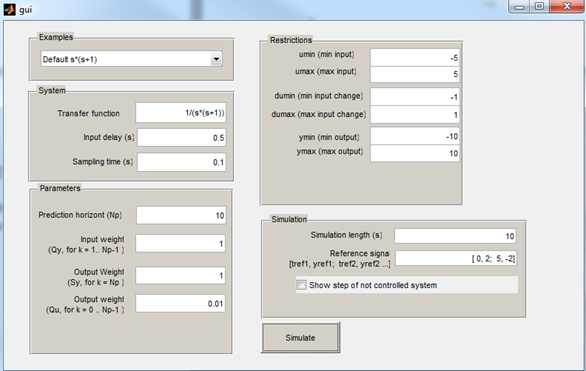
\includegraphics[width=0.99\textwidth]{08_gui.png}
\caption{Grafické rozhranie k programu na testovanie MPC algoritmu.}
\label{08_gui}
\end{figure}

a ponúka pre používateľa možnosti zadania:

\begin{itemize}
\item
  Systémových nastavení:

  \begin{itemize}
  \item
    Automatický vyplniť určité druhy systému
  \item
    Zadať akúkoľvek prechodovú funkciu v~s~alebo z~oblasti systému,
    ktorý má byť riadený
  \item
    Zadať dopravné oneskorenie systému
  \item
    ~periódu vzorkovania
  \end{itemize}
\item
  Ladiace parametre

  \begin{itemize}
  \item
    ~váha vstupu
  \item
    ~váha výstupu pre budúce hodnoty v kroku k=0 \dots N-1, N je horizont predikcie.
  \item
    ~váha výstupu pre budúcu hodnotu v kroku k=N, kde N je horizont predikcie
  \end{itemize}
\item
  Obmedzenia systému

  \begin{itemize}
  \item
    ~minimálny vstup
  \item
    ~maximálny vstup
  \item
    ~minimálna zmena vstupu
  \item
    ~maximálna zmena vstupu
  \item
    minimálny~výstup systému
  \item
    ~maximálny výstup systému
  \end{itemize}
\item
  Parametre simulácie

  \begin{itemize}
  \item
    ~čas simulácie
  \item
    ~referenčný signál zadávaný vo forme vektor dvojice hodnôt, kde prvá
    identifikuje čas, kedy ma zmena nastať a~druhá hodnota veľkosti
    skoku.
  \end{itemize}
\end{itemize}

Výstup z~grafického rozhrania po ponechaní prednastavených hodnôt sú grafy zobrazené na obrázku  \ref{09_out}.

\begin{figure}[h]
\centering
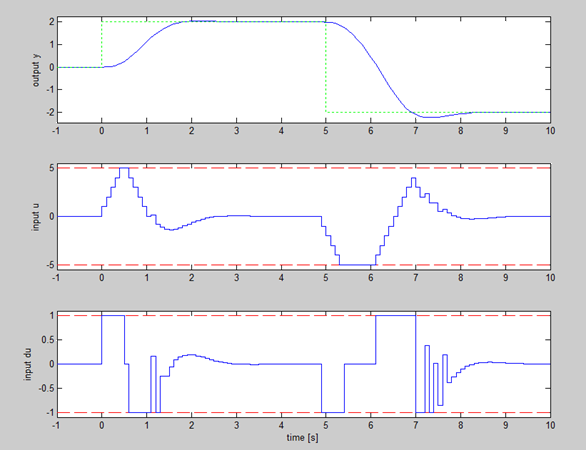
\includegraphics[width=0.99\textwidth]{09_out.png}
\caption{Časové priebehy výstupu systému, riadiaceho zásahu a zmeny riadiaceho zázsahu.}
\label{09_out}
\end{figure}


V~prvom grafe obrázku  \ref{09_out} je znázornený časový priebeh sledovania referenčnej hodnoty výstupnou veličinou. Zelenou farbou je referenčná veličina a výstupna veličina modrou.
V~druhom grafe obrázku  \ref{09_out} je znázornený
riadiaci zásah systému modrou farbou a~obmedzenia riadiaceho zásahu červenou farbou. V~treťom grafe obrázku  \ref{09_out} je znázornená zmena riadiaceho zásahu modrou farbou
a~obmedzenia červenou. Hodnotenie kvality regulácie priamymi ukazovateľmi \cite{MPC06}

\begin{itemize}
  \item Doba regulácie:
    \begin{itemize}
  		\item
    	Pre zmenu v čase 0s (zmena 1.) z hodnoty 0 na 2 je doba regulácie 2 sekundy
    	\item
    	Pre zmenu v čase 5s (zmena 2.) z hodnoty 2 na -2 je doba regulácie 3 sekundy
	\end{itemize}
  \item Preregulovanie:
    \begin{itemize}
  		\item
    	Pre zmenu 1. došlo k minimálnemu preregulovaniu.
    	\item
    	Pre zmenu 2. je preregulovanie badateľné.
	\end{itemize}  
  \item Regulačná odchýlka:
    \begin{itemize}
  		\item
    	Regulačná odchýlka je pre oba prípady 0.
	\end{itemize}   
\end{itemize}

Nie je tu porovnanie voči iným regulátorom, pretože to nie je zámerom tejto kapitoly. Kapitola slúži na demonštráciu funkčnosti predchádzajúcej teórie. Čo je však dôležité si na tomto mieste zdôrazniť je znázornenie ako vplývajú obmedzenia na riadenie systému. 

\begin{itemize}
  \item \textbf{Obmedzenie veľkosti akčného zásahu} je možné pozorovať v strednom grafe obrázku \ref{09_out} pri zmene 2. v čase 5.3 sekundy, kedy vidieť ako systém narazil na obmedzenie akčného zásahu a na tejto hodnote ostane až do času 6.1 sekundy. Ak by obmedzenie nebolo samozrejme by bola doba regulácie kratšia avšak akčný zásah bez obmedzení vo väčšine prípadov nezodpovedá realite.
  \item \textbf{Obmedzenie veľkosti zmeny akčného zásahu} je opäť možné pozorovať v strednom grafe obrázku \ref{09_out} pri obidvoch zmenách referenčného signálu. Zvýraznené to je v obrázku \ref{10_steps}. Riadiaci zásah v~tvare ,,schodov`` je dôsledkom tohto obmedzenia zmeny akčného zásahu. Z obrázku \ref{10_steps} je možné vyčítať periódu vzorkovania 0.1 sekundy, keďže je v grafe za 1 sekundu 10 zmien akčného zásahu. Prípad, že obmedzenie zmeny akčného zásahu je nastavené na hodnotu 5 (rovnaká ako obmedzenie akčného zásahu) je zobrazené na obrázku \ref{11_nosteps}.
\end{itemize}   


\begin{figure}[h]
\centering
\begin{subfigure}{.5\textwidth}
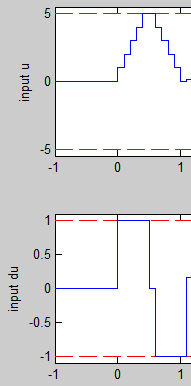
\includegraphics[width=0.5\linewidth]{10_steps.png}
\caption{Zapnuté obmedzenie}
\label{10_steps}
\end{subfigure}%
\begin{subfigure}{.5\textwidth}
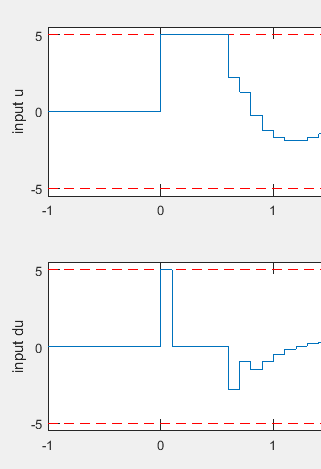
\includegraphics[width=0.7\linewidth]{11_nosteps.png}
\caption{Vypnuté obmedzenie.}
\label{11_nosteps}
\end{subfigure}
\caption{Ukážka vplyvu obmedzenia zmeny riadiaceho zásahu na časový priebeh riadiaceho zásahu.}
\end{figure}

Na základe týchto experimentov sa potvrdzujú výhody MPC regulátora, ktoré boli spomenuté v úvode ohľadne jednoduchosti zavedenia obmedzení. V tomto má MPC bližšie spojenie s reálnym systémom ako iné regulátory napr. PID, kde sa obmedzenie akčného zásahu musí špeciálne riešiť.

Ďalší nástroj na overenie MPC algoritmu je voľne stiahnuteľný
a~použiteľný v~prostredí Matlab. Názov je MPT toolbox. Je to dielo
inštitútu pre automatizáciu vo Švajčiarsku. Tento program je jeden
z~najpouživanejších v~prostredí Matlab. Nasleduje overenie algoritmu na reálnom systéme z praxe, ktorý je popísaný v nasledujúcej podkapitole. Následne je identifikovaný matematický model systému a overenie funkčnosti MPC princípov. Treba spomenúť, že overenie je stále prostredníctvom simulácie v prostredí Matlab.

\subsubsection{Popis systému riadenia plynovej turbíny}
Turbína s~výkonom 1.5MW obsahuje tri hlavné časti, menovite, kompresor,
spaľovaciu komorou a~vysokotlakovú turbínu. V~rokoch 1950 bolo
priemyselné využitie turbín významne rozšírené, kvôli jej nespočetným
výhodám. Napríklad neprítomnosť častí, ktoré by sa o~seba odierali,
nízka spotreba palív a~vysoká operačná spoľahlivosť. Prvá časť turbíny
zahŕňa stláčanie vzduchu na poskytnutie vysokého pomeru tlaku medzi
turbínou a~kompresorom, takže sa vzduch rozpína do turbíny. Zvyšovanie
teploty vzduchu spaľovaním paliva spôsobuje väčšie rozpínanie horúceho
vzduchu v~turbíne, poskytujúc tak potrebný výstupný výkon. Pre rôzne
prietoky vzduchu je limitovaný pomer vzduchu, ktorý môže byť dodaný, čo
je označované ako pomer palivo/vzduch. Tento faktor obmedzuje výstupný
výkon, ktorý môže byť dosiahnutý.~Maximálny pomer palivo/vzduch je
určený pracovnou teplotou lopatiek turbíny, ktoré sú vysoko stláčané.
Zaznamenanie možnej poruchy lopatiek je dôležitý problém pri monitoringu
a~detekcii chýb. Primárna požiadavka na riadenie je výstupný výkon, ale
neexistuje žiadny vhodný spôsob merania výkonu. Premenné súvisiace
s~výkonom sú riadené prostredníctvom riadenia generátora rýchlosti
N\textsubscript{g}, moduláciou prívodu paliva, kde N\textsubscript{g} je
funkciou výkonu generátora. Riadiaci zásah určuje množstvo paliva
dodávaného do motora, čo je funkciou uhla otvorenia klapky
\(\theta_{v}\left( \right).\) Parametre systému a~regulátora: rýchlosť
motora leží medzi 0 a~30~000 rpm (=500rps) táto premenná môže byť
považovaná za známu a~reprezentuje od 0 po 1.5MW. Vstup do systému je
náklon plynovej klapky 0-60°, čo je ekvivalent toku paliva 0-625kg/h.
Riadiaci rozsah výkonu je od 0 po plný výkon. Od 17~001-27~000 rpm
(283,35-450rps) je považovaný za stabilný stav rýchlosti generátora.\cite{MPC07}
\subsubsection{Identifikácia a riadenie systému plynovej turbíny}
Vstupné dáta na identifikáciu systému sú zobrazené na obrázku  \ref{12_data}. 

\begin{figure}[h]
\centering
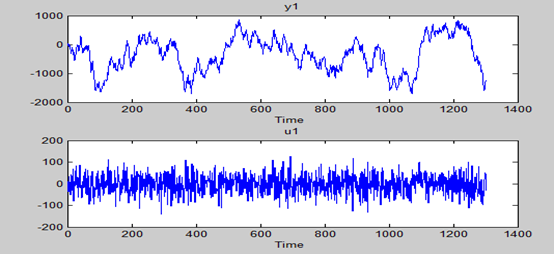
\includegraphics[width=0.9\textwidth]{12_data.png}
\caption{Časový priebeh nameraných údajov výstup a vstup systému.}
\label{12_data}
\end{figure}
Premenná y\textsubscript{1} reprezentuje výstup - otáčky motora a~u\textsubscript{1}
vstup systému - natočenie klapky. Na identifikáciu systému bol použitý Matlab nástroj \textit{ident}. Pri zisťovaní matematického modelu bolo vyskúšaných viacero metód. Najlepšie
výsledky - percento zhody nameraných a simulovaných dát dal arx model. Porovnanie nameraných a~simulovaných dát sú na
obrázku \ref{13_ident}.


\begin{figure}[h]
\centering
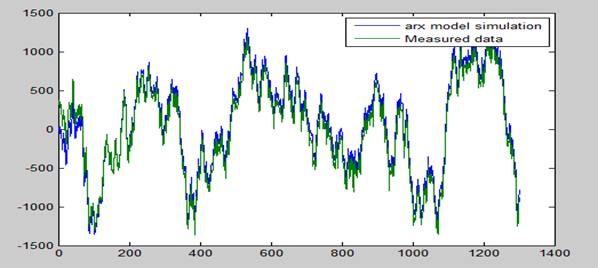
\includegraphics[width=0.9\textwidth]{13_ident.png}
\caption{Porovnanie simulovaných a nameraných údajov}
\label{13_ident}
\end{figure}
Os x predstavuje čas v sekundách a y predstavuje výstup systému. Pomocou modelu arx sa získala nasledovná prenosová funkcia

\begin{equation} \label{eq38}
\begin{split}
Gp(z) = \ \frac{Y(z)}{U(z)}
\end{split}
\end{equation}

kde
\begin{equation} \label{eq39}
\begin{split}
\text{\ Y}\left( z \right) = 2.085z^{- 1} + 0.3692z^{- 2} \\
U\left( z \right) = 1 - 0.99{13z}^{- 1} + 1.287 \times 10^{- 3}z^{- 2}
\end{split}
\end{equation}
Perióda vzorkovania je \(T_{s} = 0.25\).

Navrhnutý algoritmus bol otestovaný na reálnom systéme s~prenosovou
funkciou \ref{eq39}. Parametre simulácie sú zobrazene na obrázku \ref{15_paramt}. Časové odozvy systému s~MPC regulátorom sú
na obrázku \ref{14_simt}. Konkrétne časová odozva výstupu, v~tomto prípade
výkon motora, meraný v~rps (otáčky za sekundu) je zobrazený vo vrchnom
grafe. Vstup systému, uhol náklonu plynovej klapky meraný v~stupňoch je
v~strednom grafe a~zmena vstupu v~spodnom grafe. Všetky spomenuté
veličiny majú v~grafe modrú farbu. Zelená farba vo vrchnom grafe
predstavuje referenčný signál a~červené čiarkované čiary sú obmedzenia.

\begin{figure}[h]
\centering
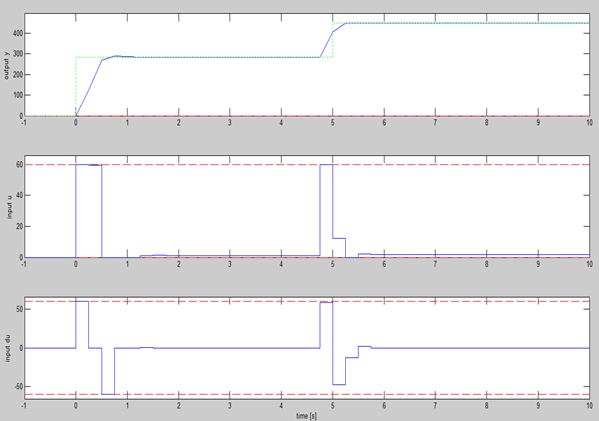
\includegraphics[width=0.9\textwidth]{14_simt.png}
\caption{Časové odozvy rýchlosti motora (v jednotkách rps) s MPC regulátorom}
\label{14_simt}
\end{figure}

\begin{figure}[h]
\centering
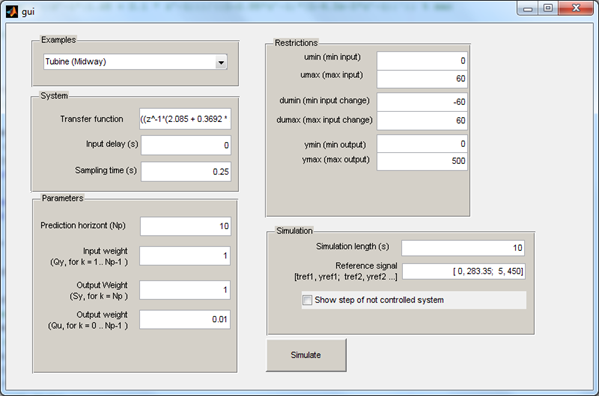
\includegraphics[width=0.9\textwidth]{15_paramt.png}
\caption{Parametre simulácie}
\label{15_paramt}
\end{figure}

renosová funkcia \ref{eq39} sa zadala do grafického rozhrania do pola
„transfer function``. Horizont predikcie bol nastavený na 10 vzoriek
dopredu. Zo simulácii vyplýva, že je to dostatočné a~efektívne, berúc do
úvahy odozvu systému a~kvalitu riadenia. Váhy boli nastavené na
prednastavené hodnoty. Obmedzenia algoritmu sú

\begin{itemize}
\item
  Na vstup 0-60 stupňov.
\item
  Zmena vstupu -60 -- 60 stupňov.
\item
  Výstup systému 0 -- 500 rps (30~000 rpm)
\end{itemize}

Referenčný signál je nastavený na hodnotu 283.35 rps v~čase 0. Po 5
sekundách je nastavený na hodnotu 450 rps.

Z~výsledkov je možné vidieť výhody prediktívneho riadenia. Keďže
prediktívny regulátor je založený na optimalizácii, je možné vidieť
minimálne akčné zásahy, čo môže viesť k~úspore spotreby.\cite{MPC08}\\
Týmto končí simulačné overovanie algoritmu MPC regulátora vytvoreného na základe teoretických princípov popísaných v úvodných kapitolách MPC regulátora a nasleduje druhá časť práce, ktorá pripraví podklady pre praktický experiment.

\section{Softvérová Architektúra}
Téma softvérovej architektúry (Software architectrue) zahŕňa veľa súčastí. Práca sa zameriava len na tie časti, ktoré vedú do problematiky internetu vecí a teda nepojednáva o všetkých aspektoch tejto problematiky. Nasleduje niekoľko definícií a vymenovanie typov aplikácii. 

\indent Softvérová architektúra je proces definovania štrukturovaného riešenia, ktoré spĺňa všetky technické a operačné požiadavky, zatiaľ čo optimalizuje bežné kvalitatívne vlastnosti ako je výkonnosť, bezpečnosť a ovládateľnosť. Zahŕňa rad rozhodnutí, ktoré sú založené na viacerých faktoroch a každé z týchto rozhodnutí môže mať značný dopad na kvalitu, výkonnosť, udržiavanie a celkový úspech aplikácie.

\indent Philippe Kruchten, Grady Booch, Kurt Bittner a Rich Reitman odvodili a vylepšili definíciu architektúry, ktorá vychádza z práce Mary Shaw a David Garlan (Shaw and Garlan 1996). Ich definícia je:

\indent Softvérová architektúra zahŕňa sadu dôležitých rozhodnutí o usporiadaní softvérového systému vrátane voľby stavebných prvkov a ich rozhraní, pomocou ktorých je systém zložený. Rozhodnutie o voľbe správania, ktoré je definované spoluprácou medzi uvedenými prvkami. Rozhodnutie o spájaní týchto štrukturálnych a behaviorálnych elementov do rozsiahlejších subsystémov a voľba architektonického štýlu, ktorý vedie toto usporiadanie. Softvérová architektúra tiež zahŕňa starosť o funkcionalitu, použiteľnosť, pružnosť, výkonnosť, možnosť znovu použitia, zrozumiteľnosť, kompromisy na ekonomické a technologické obmedzenia a tiež estetickosť. \cite{IOT02}

\indent Dôležité si je uvedomiť, že softvérová architektúra je prostriedok na vytvorenie softvérového systému avšak softvérový systém je stále len prostriedok na dosiahnutie určitého cieľa.

\indent Preto by systémy mali byť navrhované s prihliadaním na \textbf{používateľa}, \textbf{systém} (IT infraštruktúra) a \textbf{biznis ciele}, ako je zobrazené na obrázku \ref{18_arch}. Pre každú z týchto oblastí by mal byť načrtnutý kľúčový scenár a identifikované dôležité kvalitatívne vlastnosti (napríklad spoľahlivosť a škálovateľnosť) a kľúčové oblasti uspokojenia alebo neuspokojenia. Vytvoriť metriky a prihliadať na ne pri meraní úspechu v každej z oblasti, všade kde je to možné.
\cite{IOT02}
\begin{figure}[h]
\centering
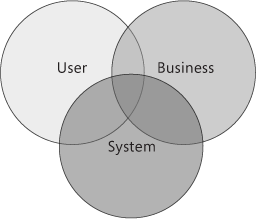
\includegraphics[width=0.3\textwidth]{18_arch.png}
\caption{Oblasti, potrebné zvažovať pri návrhu\cite{IOT02}}
\label{18_arch}
\end{figure}

\subsection{Základne typy architektúr}
Jedno z kľúčových rozhodnutí je voľba typu architektúry. Tie najpoužívanejšie sú vymenované nižšie podľa článku \cite{IOT05} napísanom na základe knihy\cite{IOT08}, ktorú napísal Mark Richards - softvér architekt s 30 ročnou skúsenosťou. V článku sa tiež uvádza, že v jednom systéme môže byť použitých viacero typov, čo je  dôležitá informácia pri návrhu.
\begin{itemize}
 \item \textbf{ N-vrstvová architektúra.} Je to jeden z najpoužívanejších prístupov, pretože je to postavené okolo databázy a veľa aplikácií v biznise prirodzene potrebujú ukladať informácie v tabuľkách. \indent Veľa z najznámejších frameworkov ako Java EE, Drupal a Express sú postavené tak, aby mali túto štruktúru na mysli, takže aplikácie, nimi vytvorené sú automaticky N-vrstvové.
\indent Zdrojový kód je usporiadaný tak, že dáta vstupujú na najvyššej úrovni a prepracujú sa cez každú vrstvu až dosiahnú najnižšiu, čo je zvyčajne databáza. Po ceste má každá vrstva svoju úlohu, ako kontrolovanie konzistencie dát alebo formátovanie dát, tak aby ostali konzistentné. Je bežné, že rôzny programátori pracujú nezávisle na jednotlivých vrstvách.
\begin{figure}[h]
\centering
\begin{subfigure}{0.5\linewidth}
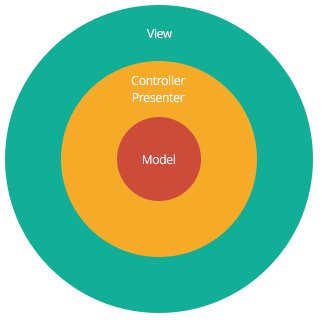
\includegraphics[width=0.9\textwidth]{25_3l.png}
\caption{3 vrstvová architektúra \cite{IOT07}}
\label{25_3l}
\end{subfigure}%
\begin{subfigure}{0.5\linewidth}
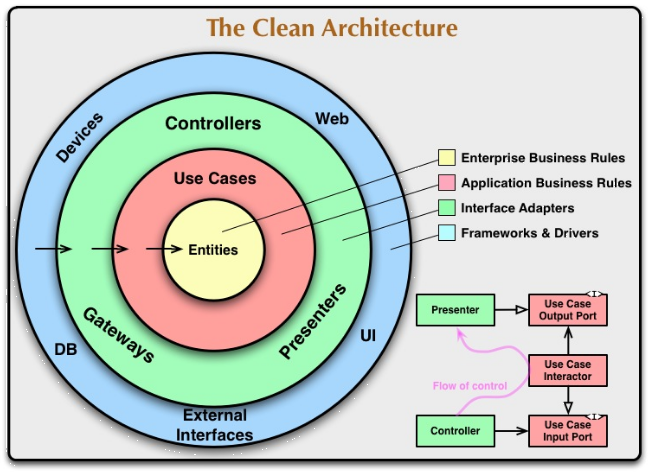
\includegraphics[width=0.9\textwidth]{24_4l.png}
\caption{4 vrstvová architektúra\cite{IOT06}}
\label{24_4l}
\end{subfigure}
\end{figure}
MVC (Model-View-Controller) štruktúra, ktorú poskytuje väčšina obľúbených frameworkov je zjavne N-vrstvová architektúra. Nad databázou je model, ktorý často obsahuje biznis logiku a informácie o type dát databáze. Na vrchu je zobrazovacia vrstva, ktorá často pozostáva z CSS, JavaScript a HTML. V strede je ovládač, ktorý má viacero pravidiel a funkcií na transformáciu dát zo zobrazovacej vrstvy do modelu.
 \item \textbf{ Architektúra riadená udalosťami.} Veľa programov trávi väčšinu času čakaním, kým sa niečo stane. Tento fakt špeciálne platí pre systémy, ktoré priamo spolupracujú  s ľuďmi, ale rovnako je to bežné aj v oblasti sietí.
\indent Architektúra riadená udalosťami pomáha spravovať uvedené fakty tak, že sa vytvorí centrálna jednotka, ktorá prijíma dáta a potom ich deleguje do samostatných modulov, ktoré dáta spracujú. Toto odovzdanie sa nazýva vygenerovanie udalosti. Udalosť je následne spracovaná kódom tzv. event-handler.
 \item \textbf{ ,,Microkernel`` architektúra.} Veľa aplikácií má základnú sadu operácií, ktoré sú znova a znova použité v iných prípadoch, ktoré závisia od aktuálneho typu dát a typu úlohy. Obľúbený nástroj na vývoj Eclipse, napríklad, najskôr otvorí súbory, pridá im poznámky, upraví ich a potom spustí pomocníka na pozadí. Nástroj je vykonávaním týchto operácií známy a s kódom napísaným v jazyku Java na jedno stlačenie tlačítka sa kód skompiluje a spustí.
\indent V tomto prípade, základný program na zobrazovanie a upravovanie súboru sú súčasťou microkernel-u. Java kompilátor je extra časť, ktorá je pridaná na podporu základných čŕt microkernel-u. Ostatní vývojári vyvinuli ďalšie časti, aby bolo možné vyvíjať aj v iných jazykoch s inými kompilátormi. Často krát sa kompilátor ani nepoužíva, ale využívajú len funkcie na úpravu súborov. 
\indent Špeciálne pridaná funkcionalita sa nazýva plug-in. Často je tento prístup nazývaný aj Plug-in architektúra.
 \item \textbf{ ,,Microservice`` architektúra.} Softvér môže byť ako malý slon. Keď je malý je milý a zábavný, ale keď dospeje, je ťažké ho viesť a bráni sa zmene. Návrh Microservice architektúry pomáha vývojárom predísť tomu, aby sa z ich malých programov stali ťažkopádne, monolitické a neflexibilné programy. Preto na miesto vytvárania jedného veľkého programu je cieľ vytvoriť množstvo rozličných malých programov a vždy keď chce niekto pridať funkcionalitu, tak vždy pridať malý program.
\indent Tento prístup je podobný Microkernel 
a udalosťami riadenému prístupu, ale je používaný zvyčajne, keď rozličné úlohy sú ľahko oddeliteľné. Vo veľa prípadoch, rozličné úlohy môžu vyžadovať rôzny čas na spracovanie a môžu sa líšiť v spôsobe použitia. Napríklad servery spoločnosti Netflix, ktoré poskytujú obsah zákazníkom (filmy a videá) majú oveľa väčšiu záťaž v piatok a sobotu večer, takže musia byť pripravený zvýšiť výpočtové a sieťové kapacity. Servery, ktoré sledujú vrátenie požičaných DVD, na druhej strane, robia svoju robotu cez týždeň hneď ako pošta doručí príchodzie zásielky. Ak sa to implementuje ako oddelené služby, Netflix cloud ich môže nezávisle škálovať podľa dopytu.
 \item \textbf{ ,,Space-based`` architektúra.} Veľa aplikácií, ktoré sú postavené okolo databázy a fungujú správne pokiaľ databáza stíha spracovávať záťaž. Keď však databáza prestane stíhať zapisovať veľa transakcií, celá aplikácia spadne.
 \indent ,,Space-based`` architektúra je navrhnutá tak, aby predišla zlyhaniu pri veľkej záťaži rozložením spracovania a ukladania na viacero serverov. Dáta aj zodpovednosť za možnosť zavolania služby sú rozdistribuované na viacero uzlov. Niektorí architekti používajú širokejší pojem ,,cloud`` architektúra. Táto architektúra podporuje prípady, kedy je ťažké predikovať nárast požiadaviek, ktorý by databáza nestíhala spracovávať. 
\indent Uchovávanie informácie v RAM umožňuje vykonávať veľa úloh rýchlejšie a zjednodušuje zdieľanie medzi uzlami. Avšak distribuovaná architektúra robí niektoré analýzy komplikovanejšími. Výpočet, ktorý musí prebehnúť cez všetky dáta, napríklad výpočet priemeru alebo vytváranie štatistickej analýzy musí byť rozdelený na podúlohy cez všetky uzly a keď skončia zoskupenie dát je potrebné. 
\end{itemize}

\subsection{Základné typy aplikácií}
Ďalšie z kľúčových rozhodnutí je voľba typu aplikácie. Na výber podľa  článku \cite{IOT03} sú:
\begin{itemize}
\item
 \textbf{Mobilná aplikácia obrázok \ref{19_mob}.} Aplikácie tohto typu môžu byť vyvíjané ako tenký alebo tučný klient. Mobilná aplikácia vo forme tučného klienta môže podporovať scenáre bez pripojenia alebo s občasným pripojením. Webové aplikácie alebo tenkí klienti podporujú iba scenáre s pripojením. Zdroje, ktorými disponujú mobilné zariadenia sa často ukazujú ako obmedzenie pri návrhu mobilných aplikácií. \\
Výhody: 
 \begin{itemize}
   \item  Podpora mobilných zariadení.
   \item  Dostupnosť a jednoduchosť použitia pre používateľov mimo kancelárie.
   \item  Podpora pre scenáre bez pripojenia a s občasným pripojením.   
 \end{itemize}
Na zváženie: 
 \begin{itemize}
   \item Limity ohľadne zadávania údajov a navigácie v aplikácii.
   \item Limitovaná šírka zobrazovanej plochy.   
 \end{itemize}
 
\item
 \textbf{Tučná klientská aplikácia obrázok \ref{20_cli}.} Aplikácie tohto typu sú zvyčajne vyvíjané ako stand-alone aplikácie s grafickým rozhraním, ktoré zobrazuje dáta prostredníctvom rôznych ovládacích prvkov. Tuční klienti sú väčšinou navrhnutí na scenáre bez pripojenia alebo s občasným pripojením, keď potrebujú prístup k vzdialeným dátam alebo funkcionalite. \\
Výhody: 
 \begin{itemize}
   \item  Možnosť využívať zdroje klienta.
   \item  Lepšia odozva, bohatá funkčnosť používateľského rozhrania a lepší používateľský zážitok.
   \item  Dynamická a responzívna interakcia.
   \item Podpora scenárov bez pripojenia alebo s dočasným pripojením.   
 \end{itemize}
Na zváženie: 
 \begin{itemize}
   \item Komplikovanejšie nasadenie. Avšak existuje množstvo inštalačných možnosti ako ClickOnce, Windows Installer a XCOPY je dostupných.
   \item Problém s nasadzovaním nových verzií v čase.   
   \item Závislé od platformy.
 \end{itemize}

\begin{figure}[h]
\centering
\begin{subfigure}{0.5\linewidth}
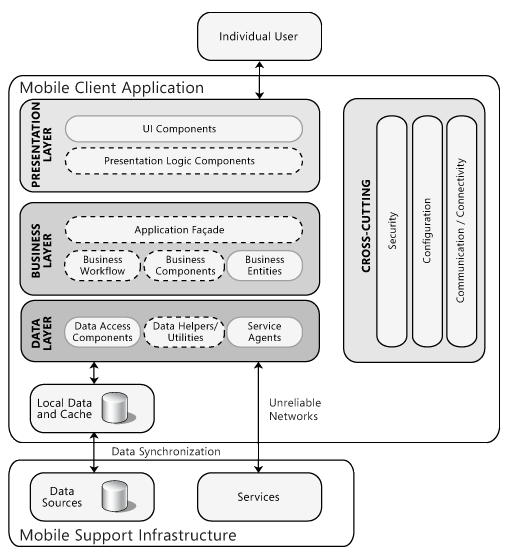
\includegraphics[width=0.9\textwidth]{19_mob.png}
\caption{Mobilná aplikácia \cite{IOT03}}
\label{19_mob}
\end{subfigure}%
\begin{subfigure}{0.5\linewidth}
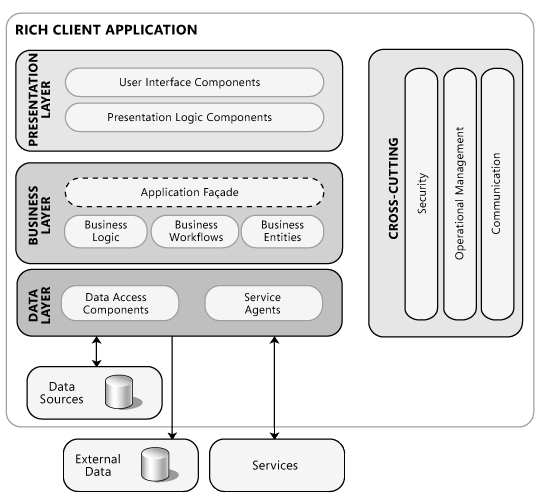
\includegraphics[width=0.9\textwidth]{20_cli.png}
\caption{Clientská aplikácia \cite{IOT03}}
\label{20_cli}
\end{subfigure}
\caption{}
\end{figure}

 
\item
 \textbf{Tučná internetová aplikácia obrázok \ref{21_ri}.} Aplikácie tohto typu sú vyvíjané tak, aby podporovali viacero platforiem a prehliadačov tak, že zobrazujú multimédia alebo iný grafický obsah. Tučné internetové aplikácie bežia v prehliadači, čím sú obmedzený pristupovať k niektorým zdrojom klienta. \\
Výhody: 
 \begin{itemize}
   \item  Rovnaké schopnosti užívateľského rozhrania ako tuční klienti.
   \item  Podpora multimédií a stream medií
   \item  Jednoduché nasadzovanie  s rovnakými možnosťami distribúcie ako weboví klienti. 
   \item Jednoduchý upgrade na novú verziu.
   \item Podpora cez väčšinu platforiem a prehliadačov. 
 \end{itemize}
Na zváženie: 
 \begin{itemize}
   \item Kladie vyššie nároky na klienta ako webové aplikácie.
   \item Obmedzenia na využívanie zdrojov klienta oproti tučnej klientskej aplikácii. 
   \item Vyžaduje mať na klientovi nasadený vhodný runtime framework.
 \end{itemize} 
 
  \item
  \textbf{Webová aplikácia obrázok \ref{23_web}.} Aplikácie tohoto typu zvyčajne podporujú scenáre s pripojením, podporujú viacero prehliadačov, ktoré bežia na rôznych operačných systémoch.\\
Výhody: 
 \begin{itemize}
   \item Široká dostupnosť pre väčšinu platforiem a užívateľské rozhranie je vytvárané prostredníctvom štandardov.
   \item Jednoduchosť nasadenia a správy zmien.
 \end{itemize}
Na zváženie: 
 \begin{itemize}
   \item Závislé od nepretržitého sieťového spojenia.
   \item Komplikácie s poskytnutím bohatého (rich) užívateľského rozhrania.
 \end{itemize}  
 
\begin{figure}[h]
\centering
\begin{subfigure}{0.5\linewidth}
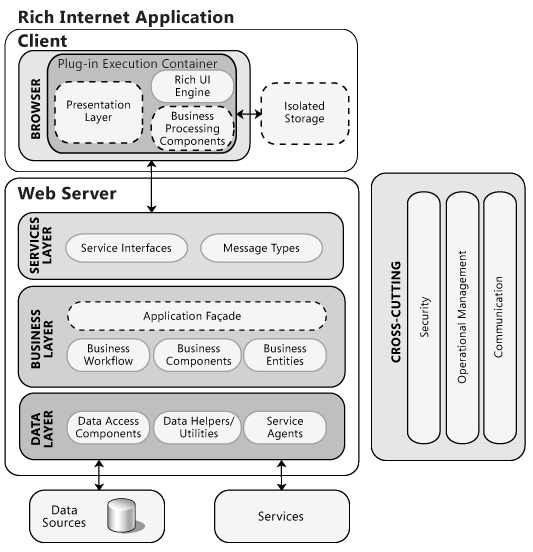
\includegraphics[width=0.9\textwidth]{21_ri.png}
\caption{Tučná internet aplikácia \cite{IOT03}}
\label{21_ri}
\end{subfigure}%
\begin{subfigure}{0.5\linewidth}
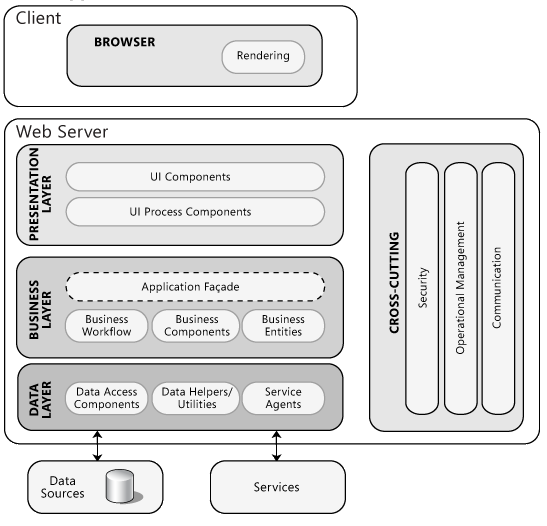
\includegraphics[width=0.9\textwidth]{23_web.png}
\caption{Web aplikácia \cite{IOT03}}
\label{23_web}
\end{subfigure}
\caption{}
\end{figure}

 \item
  \textbf{Servisná aplikácia obrázok \ref{22_ser}.} Služby vystavujú zdieľanú biznis funkcionalitu a umožňujú klientom pristupovať k nim z lokálneho alebo vzdialeného systému. Operácie služieb sú volané prostredníctvom správ založených na XML schémach, posielaných cez transportnú vrstvu. Cieľom týchto aplikácií je dosiahnutie voľných väzieb medzi klientom a serverom. \\
Výhody: 
 \begin{itemize}
   \item Interakcie medzi klientom a serverom je prostredníctvom voľných väzieb.
   \item Môže byť použitá rôznymi nezávislými aplikáciami.
   \item Podpora pre interoperabilitu.
 \end{itemize}
Na zváženie: 
 \begin{itemize}
   \item Nie je podpora pomocou užívateľského rozhrania.
   \item Závisí od sieťového pripojenia.
 \end{itemize} 

\begin{figure}[h]
\centering
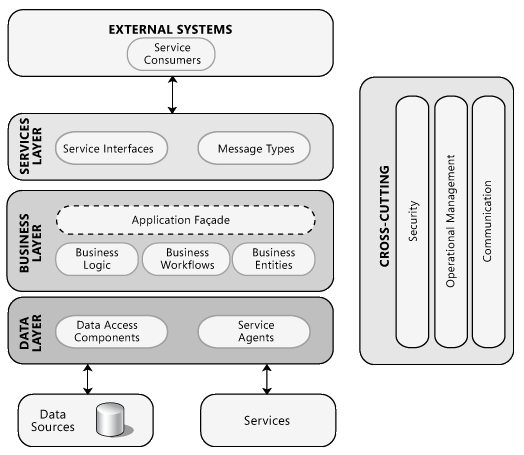
\includegraphics[width=0.75\textwidth]{22_ser.png}
\caption{Aplikácia poskytujúca službu \cite{IOT03}}
\label{22_ser}
\end{figure} 
    
\end{itemize}
\subsubsection{Servisná aplikácia}
Servisným aplikáciam je v práci venovaná samostatná kapitola, pretože v implementácii je použitý takýto typ aplikácie. Servisné aplikácie majú svoje miesto vo väčšine enterprise architektúr.  Enterprise architektúra je koncepčný návrh, ktorý definuje štruktúru a prevádzkovanie spoločnosti. Zámer enterprise architektúry je rozhodnúť ako môže organizácia najefektívnejšie dosiahnuť aktuálne a budúce ciele \cite{IOT09}. Inými slovami ide o  architektúru podnikových informačných systémov, ktoré zvyčajne pozostávajú z viacerých súčasti. Príkladom týchto súčasti môže byť:
\begin{itemize}
  \item  \textbf{CRM aplikácia.} Podľa APICS slovníka \cite{IOT10} je CRM definované ako úložisko a analýza informácií navrhované pre podporu predajných a marketingových rozhodnutí, na pochopenie a podporu potrieb existujúcich a potenciálnych zákazníkov. Zahŕňa správu užívateľských účtov, môže zahŕňať katalóg produktov, zadávanie objednávky, spracovanie a úpravu platieb a iné funkcie.\cite{IOT11}. Všetky, ktoré sú v definícii uvedené ako ,,môže zahŕňať``, závisí od konkrétnej implementácie, či dané funkcionality CRM obsahuje alebo nie. Pretože každá zo spomenutých funkcionalít môže byť ako samostatná servisná aplikácia. V tejto práci sú uvedené ako samostatné časti a CRM sa tu obmedzí na správu užívateľských účtov.
  \item  \textbf{Katalóg produktov.} Na manažovanie závislosti medzi produktami a ovplyvňovanie typov zliav a teda výpočet ceny za produkty býva v podnikoch samostatná aplikácia
 \item  \textbf{Účtovná aplikácia.} Aplikácia na vedenie účtovníctva
 \item  \textbf{Správa majetku.} Aplikácia na správu majetku. 
  \item  \textbf{ERP aplikácia.} (Plánovanie zdrojov v podniku je pojem používaný v priemysle pre širokú škálu činností, ktoré pomáhajú organizácii spravovať jej biznis. Dôležitý cieľ je pomôcť, aby tok informácií bol nastavený tak, že biznis rozhodnutia môžu byť robené na základe poskytnutých dát. ERP aplikácie sú robené tak, aby zbierali a zatrieďovali dáta z rôznych úrovni organizácie a poskytovali tak manažmentu náhľad na kľúčové ukazovatele výkonnosti tzv. KPIs v reálnom čase.\cite{IOT12} 
\end{itemize} 
Súčastí môže byť samozrejme viac a každá organizácia si podľa svojich potrieb vyberá tie  súčasti, ktoré potrebuje. Väčšina spomenutých súčasti je dodávaná ako servisná aplikácia. Aplikácie medzi sebou môžu komunikovať prostredníctvom vystavených rozhraní. Pri malom počte vystavených rozhraní sa často používa \textbf{Point to Point \ref{26_p2p}} architektúra, kedy neexistuje centrálny bod vystavenia služby, ale ak ktorákoľvek aplikácia potrebuje zavolať inú, tak ju priamo zavolá. Takýto prístup je však krátkozraký, lebo prax ukazuje, že počet vystavených služieb časom vždy pribúda, preto je dnes rozšírené použivať tzv. SOA - \textbf{Service oriented architektúru \ref{27_soa}} s centrálnym bodom vystavovania služieb tzv. ESB - Enterprise service bus.
\begin{figure}[h]
\centering
\begin{subfigure}{0.5\linewidth}
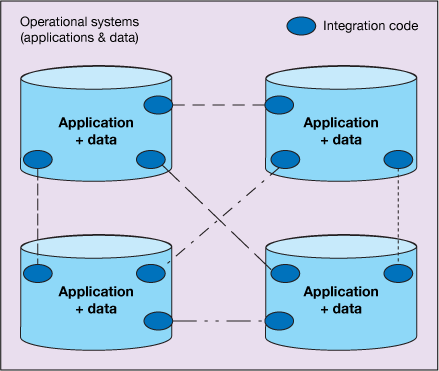
\includegraphics[width=0.8\textwidth]{26_p2p.png}
\caption{Point to Point \cite{IOT13}}
\label{26_p2p}
\end{subfigure}%
\begin{subfigure}{0.5\linewidth}
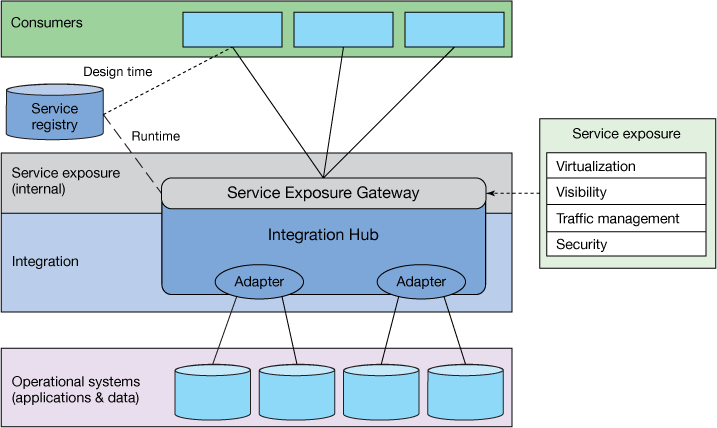
\includegraphics[width=1.1\textwidth]{27_soa.png}
\caption{SOA \cite{IOT13}}
\label{27_soa}
\end{subfigure}
\end{figure}
Existuje viacero spôsobov ako SOA implementovať. 
\begin{itemize}
 \item Najznámejší spôsob implementácie SOA, ktorí dnes používa väčšina užívateľov informačných technológií je implementácia protokolu WWW - \textbf{World Wide Web} v skratke často označovaný len WEB. 
\begin{figure}[h]
\centering

\includegraphics[width=0.75\textwidth]{28_web.png}
\caption{WWW \cite{IOT14}}
\label{28_web}
\end{figure} 
Obrázok \ref{28_web} znázorňuje princíp fungovania. Prehliadač (web browser) je v pozícii klienta, konzumera služby, ktorú poskytuje Web Server. Web Server je označenie takého počítača, na ktorom beží servisná aplikácia, ktorá vie na základe definovaných pravidiel poskytnúť požadovaný obsah. Najpoužívanejšie aplikácie, ktoré z počítača spravia web server,  v čase písania práce, z prieskumu robenom vo februári 2016 \cite{IOT15} sú Apache, Nginx, Microsoft IIS. Ich preferencie striedavo kolíšu podľa úspechu najnovších verzií. Pod službou sa v tomto prípade rozumie poskytnutie HTML dokumentu prostredníctvom aplikačného komunikačného protokolu HTTP.
\item Ďalší rozšírený protokol, ktorý implementuje SOA architektúru je \textbf{protokol SOAP}. Princíp fungovania je na obrázku \ref{29_soap}.
\begin{figure}[h]
\centering
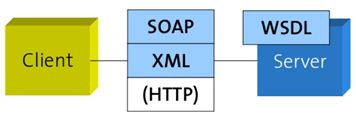
\includegraphics[width=0.75\textwidth]{29_soap.png}
\caption{SOAP \cite{IOT14}}
\label{29_soap}
\end{figure} 
Klient je v tomto prípade generickejší. Zvyčajne je to aplikácia, ktorá má XML parser (prekladač) a schopnosť komunikovať po sieti HTTP protokolom. Rovnako server je generickejší. SOAP je v tomto prípade pre server ,,len`` príručka ako službu vystaviť. Pod službou sa rozumie vystavenie RPC (remote procedure call), čo znamená umožnenie volania vzdialenej procedúry. Čo bude procedúra robiť je plne v rukách programátora. Aj v SOAP je pre transportnú vrstvu použitý HTTP protokol, obsahom správ sú XML objekty so špecifickým tvarom, ktorý SOAP definuje. Postup komunikácie je taký, že klient vytvorí XML objekt v ktorom definuje vstupné parametre do volania vzdialenej procedúry odošle požiadavku, na serveri sa vykoná procedúra a do odpovede sa pošle výsledok spracovania vzdialenej procedúry vo forme XML objektu, ktorý klient spracuje a na základe toho vie ako volanie dopadlo. 
Medzi najväčšie výhody tohto protokolu patrí možnosť striktnej validácie správnosti formátu správ, ktoré si klient a server vymieňajú. Formát správ a operácie, ktoré server poskytuje sú zadefinované vo WSDL dokumente. 
 \item Ostatná implementácia SOA architektúry uvádzaná v tejto práci je \textbf{architektonický štýl REST}. Možností samozrejme existuje viacero, ale ako bolo na začiatku tejto kapitoly uvedené, cieľom je pripraviť podklad pre vysvetlenie Internetu vecí. REST je skratka od REpresentational State Transfer. Ako je možné vidieť na obrázku \ref{30_rest} aj tu vystupuje generický klient a generický server ako v prípade SOAP protokolu.
\begin{figure}[h]
\centering
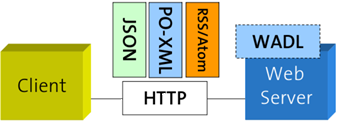
\includegraphics[width=0.75\textwidth]{30_rest.png}
\caption{REST \cite{IOT14}}
\label{30_rest}
\end{figure} 
Základný rozdiel oproti SOAP je, že HTTP je využívaný nie len ako transportný protokol, ale ako aplikačný protokol, takže sa využíva celý jeho potenciál. V praxi to znamená, že operácie, ktoré server poskytuje sú unifikované HTTP protokolom a nie je nutné, aby ich klient vyťahoval z WSDL dokumentu. Ďalšia výhoda, že HTTP je využívaný ako aplikačný protokol je, možnosť definovania aký obsah server pošle. Nie je teda obmedzenie na XML dokumenty, ale je možnosť posielať JSON objekty, binárne objekty a všetky ostatné typy správ podporované HTTP protokolom. Z uvedeného tiež vyplýva, že klientom môže byť samotný prehliadač respektíve implementácia klienta sa značne zjednodušuje. Možnosť posielať JSON objekty tiež napomáha zjednodušeniu klienta, ktorý, ak sa hovorí o web aplikácii, je zvyčajne napísaný v jazyku Javascript. Takže preklad posielanej správy na dátový typ klienta je priamočiary, bez používania ďalšieho prekladača. 
\end{itemize}
Kvôli uvedeným vlastnostiam je používanie REST rozhrania s JSON objektom ako formátom správ rozšírené pri tvorbe servisnej aplikácie, ktorá poskytuje rozhranie pre webovú aplikáciu. Okrem využívania servisných aplikácii v enterprise architektúrach podnikov je tento typ vo veľkom využívaný aj v IoT prostredí. Preto sa pri implementácii zvolil takýto typ rozhrania.
\subsection{Internet vecí - IoT}
Organizácia IEEE vydala celý dokument  s názvom ,,Smerom k definícii Internetu vecí``. Cieľom dokumentu je podať plnohodnotná definíciu IoT v rozmedzí od malých lokálnych systémov obmedzených na konkrétnu lokalitu až po globálny systém, ktorý je distribuovaný a poskladaný z komplexných systémov. V dokumente je možnosť nájsť prehľad základných požiadaviek na architektúru IoT \cite{IOT16}.
Podľa spoločnosti Gartner, ktorá je svetový líder v oblasti výskumu informačných technológií je IoT sieť fyzických objektov, ktoré majú vstavanú technológiu na komunikovanie a snímanie alebo interakciu s ich vnútornými stavmi alebo vonkajším prostredím \cite{IOT17}. 
Ešte definícia podľa stránky Techopedia: IoT je koncept, ktorý popisuje budúcnosť, kde každodenné fyzické objekty budú pripojené do internetu a budú sa vedieť sami identifikovať iným zariadeniam. Pojem je úzko spojený s RFID technológiou ako spôsobom komunikácie, aj keď to môže zahŕňať iné technológie na snímanie, bezdrôtové technológie alebo QR kódy.
\indent IoT je významné, pretože ak objekt sa vie sám digitálne reprezentovať stáva sa z neho niečo viac ako objekt samotný. Objekt sa už nevzťahuje len na nás, ale je spojený s okolitými objektami a dátami v databázach. Keď veľa objektov spolupracuje, je možné to nazvať ako inteligencia okolitého prostredia ,,ambient intelligence`` \cite{IOT18}.
Viacero ďalších technologických spoločností majú ich definíciu. Cieľom tejto práce nie vytvoriť ďalšiu definíciu, ale identifikovať spoločné črty väčšiny definícií. 
\begin{itemize}
 \item Prvá základná črta definícii je, že v nej vystupujú objekty, ktoré môžu \textbf{snímať a ovplyvňovať okolie}. Na dosiahnutie tejto črty je potrebné, aby objekty mali senzory a akčné členy, čo je jeden z hlavných záujmov odboru automatizácia, pre ktorý to nie je nič nové.    Dostupnosť a klesajúca cena snímačov a akčných členov umožňuje ich umiestňovanie aj na objekty mimo priemyslu, čo otvára priestor pre Internet vecí. 
 \item Druhá základná črta definícii je \textbf{prepojenie}. Opäť v automatizácii a priemysle to nie je nič nové, veď koľko priemyselných štandardov rieši prepojenie senzorov a akčných členov na výrobných linkách po celom svete. Hnacou silou rozvíjajúceho sa Internetu vecí sú nové možnosti drôtového a bezdrôtového pripojenia dostupné pre koncových používateľov, klesajúce náklady na prevádzku sietí a klesajúca cena zariadení, ktoré umožňujú zber a posielanie dát do dátových centier nazývaných - edge device, gateway alebo agregátor.
 \item Ďalšia spoločná črta je vyústením dvoch predošlých a to \textbf{vytváranie inteligentného prostredia}. Keď bežné objekty vedia snímať rôzne fyzikálne veličiny, zosnímané hodnoty prostredníctvom pripojenia  môžu poslať prostredníctvom agregátora do dátového centra, v dátovom centre sú hodnoty zoskupené a pripravené na urobenie analýz a štatistík, na základe ktorých, ak je možné robiť rozhodnutia v reálnom čase alebo kvázi reálnom čase, tak je spätne možnosť ovplyvniť akčný člen, čo vo veľkom môže znamenať vytvorenie inteligentného prostredia. Zabezpečenie tejto črty je predmetom oblasti ukladania a spracovania dát. V tomto bode sa IoT často spája s pojmom Big Data. Definícia tohto pojmu má viacero verzií podobne ako definícia IoT. Zvolila sa aspoň jedna od spoločnosti Gartner pre ilustráciu. Big data sú informácie veľkého objemu, veľkej rýchlosti a/alebo veľkej variability, ktoré si vyžadujú rentabilné, inovatívne formy spracovania informácii, ktoré umožňujú väčší náhľad, napomáhať rozhodovaniu a automatizácii procesov \cite{IOT19}.
\end{itemize}
Zhrnutie technológii, ktoré môže IoT zhŕňať je ďalej na obrázku \ref{31_iot}.
\begin{figure}[h]
\centering
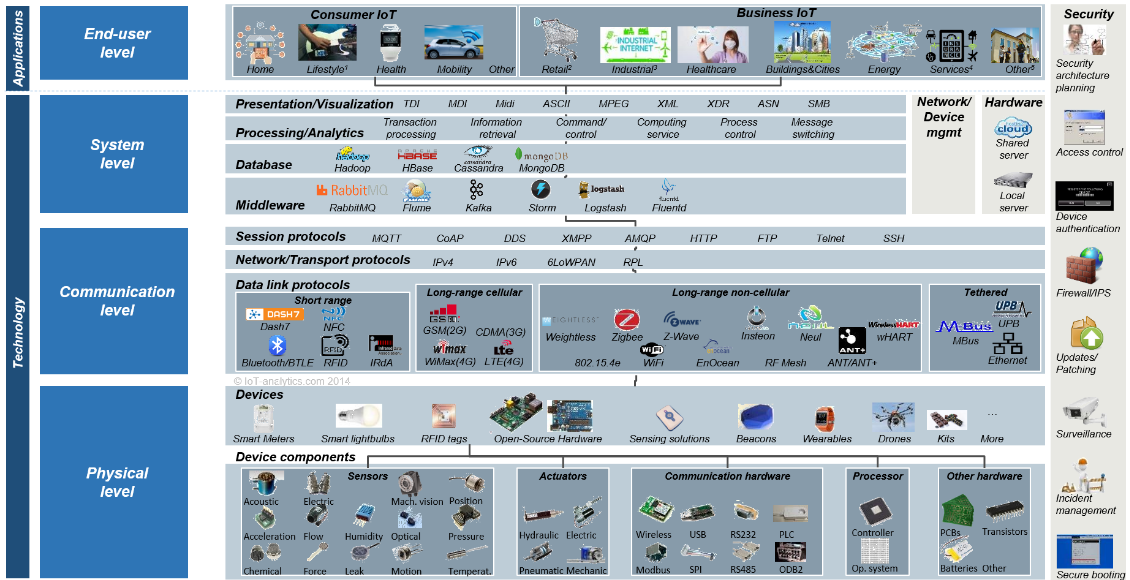
\includegraphics[width=0.99\textwidth]{31_iot.png}
\caption{IoT súhrn techológií \cite{IOT20}}
\label{31_iot}
\end{figure} 
V čom sa IoT líši od tradičnej architektúry priemyselných systémov je znázornené na obrázkoch \ref{32_iotA} a \ref{32_iotB}.

\begin{figure}[h]
\centering
\begin{subfigure}{0.5\linewidth}
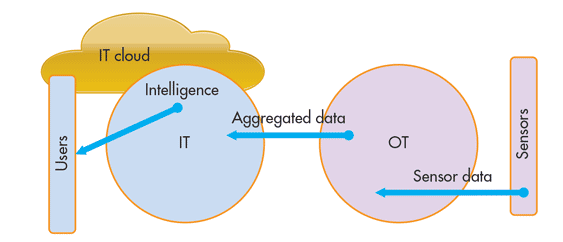
\includegraphics[width=0.9\textwidth]{32_iotA.png}
\caption{Tradičná architektúra \cite{IOT21}}
\label{32_iotA}
\end{subfigure}%
\begin{subfigure}{0.5\linewidth}
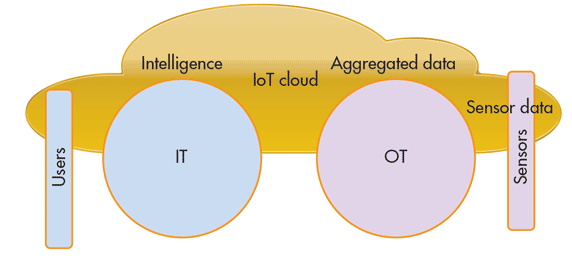
\includegraphics[width=0.9\textwidth]{32_iotB.png}
\caption{IoT architektúra \cite{IOT21}}
\label{32_iotB}
\end{subfigure}
\caption{}
\end{figure}
Tradičná priemyselná architektúra jednoducho používa vstavaný softvér na platforme obslužných technológií (Operational Technology - OT) na posunutie dát do platformy informačných technológií (Information Technology - IT), ktorá vie robiť, analýzu dát, poskytovať ich používateľovi aj vystavovať do cloud prostredia. IoT architektúra posúva väčšiu časť inteligencie systému z IT strany do OT strany. Toto umožňujú mikroprocesory a vstavané platformy s jednoduchým prístupom do cloud prostredia a rovnako s jednoduchým prístupom ku autorizovaným zariadeniam a používateľom. \cite{IOT21}. 
\indent Základné ciele IoT architektúr je zosnímané dáta čo najskôr, najbezpečnejšie a najspoľahlivejšie poslať ďalej na miesto, kde môžu prejsť analýzou, či už je to cloud alebo dosť často to býva aj samotný agregátor, ktorý má dostatočný výkon na určitý druh analýz a na základe analýzy ovplyvniť akčné členy, aby sa optimalizoval proces, náklady, zdroje atď. Veľké firmy typu Microsoft, Amazon, HP pripravili svoje platformy, ktoré sa líšia v použitých technológiách, ale princíp ostáva rovnaký. Na demonštráciu sa uvádza porovnanie dvoch hotových platforiem Azure IOT HUB od Microsoft a AWS IOT od Amazonu v tabuľke \ref{table:1} a na obrázku \ref{33_aa}.
\begin{table}[h!]
\centering
 \caption{Porovnanie dvoch IOT platforiem \cite{IOT22} }
 \begin{tabular}{ |p{4cm}|p{5.5cm}p{5.5cm}| } 
 \hline
 Produkty & MS AZURE IOT HUB & AMAZON AWS IOT \\ 
 \hline\hline
 Protokoly & HTTP, AMQP, MQTT, vlastné protokoly & HTTP, MQTT  \\ 
 \hline
 Komunikačné vzory & Diaľkové meranie, príkazy & Diaľkové meranie, príkazy \\
 \hline
 Certifikované platformy &  Intel, Raspberry Pi 2, Freescale, Texas Instruments, MinnowBoard, BeagleBoard, Seeed, resin.io & 
Broadcom, Marvell, Renesas, Texas Instruments, Microchip, Intel, Mediatek, Qualcomm, Seeed, BeagleBoard \\
 \hline
 SDK/jazyky & 	.Net, Java, C, NodeJS & C, NodeJS \\
 \hline
\end{tabular}
\label{table:1}
\end{table}

\begin{figure}[h]
\centering
\begin{subfigure}[b]{0.8\textwidth}
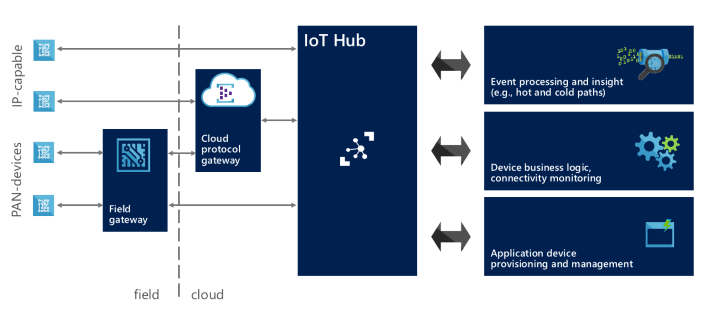
\includegraphics[width=1\linewidth]{33_azure.png}
\caption{Azure IOT HUB \cite{IOT22}}
\label{33_azure}
\end{subfigure}
\begin{subfigure}[b]{0.8\textwidth}
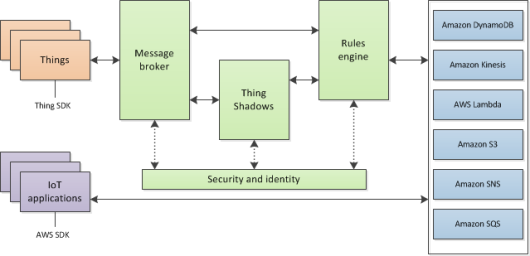
\includegraphics[width=1\linewidth]{33_aws.png}
\caption{AWS IOT \cite{IOT22}}
\label{33_aws}
\end{subfigure}
\caption{}
\label{33_aa}
\end{figure}
\indent Na portály Devexperience a stránke \cite{IOT22}, kde bolo porovnanie vykonané, definujú tieto súčasti IoT architektúry: \\
\indent Kompletné IoT riešenie pozostáva z viacero častí. Ako prvé je potrebné prijať všetky udalosti a dáta poslané zo zariadení a to je tak veľký problém, lebo v dobe internetu vecí je potrebné myslieť na škalovateľnosť v stovkách, tisíckach, miliónoch a ...  miliardách zariadení. Preto je potrebné mať \textbf{prijímací} (ingestion) systém, ktorý je schopný spracovať dáta veľmi rýchlo bez spomalenia celého procesu. Takto sa nazýva komunikačný vzor\textbf{ diaľkové meranie}. \\
\indent Po získaní dát, prijímací systém ich musí poskytnúť biznis pravidlovému systému. V spomenutých riešeniach môže byť použitá tzv. horúca cesta na analýzu dát ako tok dát v reálnom čase a tzv. studená cesta pre ukladanie dát pre budúce analýzy. Je možné to považovať za Big Data problém. Obidve cesty môžu vystaviť informácie konečnému používateľovi, ktorý môže sledovať, čo sa zo zariadeniami v reálnom svete deje. Rovnaká informácia je  užitočná pre systém strojového učenia, ktorý môže pri prediktívnej analýze napomôcť pochopiť ako sa dáta môžu vyvíjať v budúcnosti na základe aktuálnych hodnôt. \\
\indent Rovnako sa nesmie zabudnúť na opačnú cestu z cloud systému do zariadení. Vo väčšine prípadov na interakciu s nimi je potrebný vzor \textbf{príkazy} a \textbf{notifikácie}. Pomocou príkazov je možné komunikovať so zariadeniami, takže môžu vykonávať nejaké úkony. Pomocou notifikácií je možné poskytnúť zariadeniam informácie, ktoré potrebujú počas behu. Na zabezpečenie príkazov a notifikácií na komunikáciu s koncovými zariadeniami sa často používajú tzv. brány na komunikáciu zo zariadenia do cloudu a naopak často označovaný ako Cloud gateway. \\
\indent Všetky zariadenia by boli schopné pristupovať na Cloud gateway, keby boli pripojené pomocou ethernetových sietí s podporou TCP/IP protokolu. Pre zariadenia s obmedzením na prostriedky s využitím PAN (Personal Area Network) protokolov (napríklad Bluetooth, Zigbee, Z-Wave, rovnako je možné uvažovať na AllJoyn frameworkom) je potrebné uvažovať nad tzv. field gateway, ktorý vystupuje ako lokálna brána na prístup do cloud priestoru. Táto brána má úlohu prekladača protokolov a môže zabezpečovať lokálne ukladanie, filtrovanie a spracovanie úkonov, keď prídu dáta pred tým ako sa pošlú do cloud. Samozrejme to môže byť vstupný bod pre lokálny systém na prijímanie príkazov a notifikácii poslaných z cloud a smerovaných na zariadenia. \cite{IOT22}
Cieľom porovnania nie je zaoberať sa detailami implementácie jednotlivých riešení, ale poukázať na principiálnu podobnosť architektúr. Obrázok \ref{34_iot_fin} zovšeobecňuje a znázorňuje všetky možnosti zapojenia hlavných súčastí IoT riešení, ktoré sú uvedené v predošlej citácií a rovnako sa uvádzajú vo väčšine literatúr.
\begin{figure}[h]
\centering
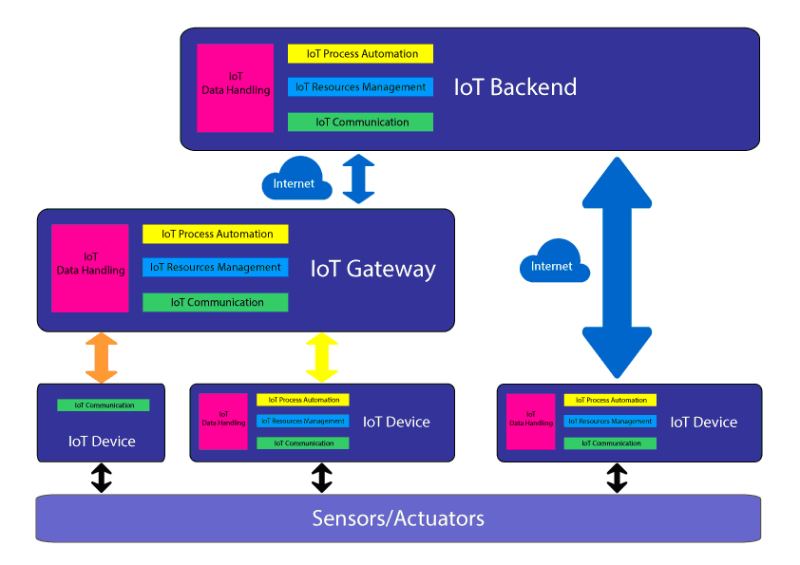
\includegraphics[width=0.99\textwidth]{34_iot_fin.png}
\caption{IoT súčasti - všeobecne\cite{IOT23}}
\label{34_iot_fin}
\end{figure} 
\subsubsection{Oblasti využitia}
Po zadefinovaní hlavných súčasti architektúry IoT riešení, práca popisuje oblasti využitia s detailným zameraním na oblasť inteligentných domácností. Ako podklad pre vymenovanie je dokument \cite{IOT24}.
\begin{itemize}
\item IT a siete - verejné, podnikové (PC, router, switch, pobočkové ústredne, ...).
\item Digitálna a verejná bezpečnosť - verejné osvetlenie, kamerové systémy...
\item Obchod - digitálne popisky, registračné pokladnice, ... 
\item Doprava - lode, lietadla, autá, mýta, ...
\item Priemysel - distribučné siete, automatizácia zdrojov, ...
\item Zdravotná starostlivosť - telemedicína a sledovanie pacientov, ...
\item Energetika - optimalizácia dopytu a ponuky, podpora efektivity alternatívnych zdrojov, ...
\item Komerčné budovy - správa budov, úspora na prevádzkovanie, ...
\item Domácnosť a spotrebiteľ - pohodlie a zábava, spotrebiče, ...
\end{itemize}

 
TODO: Inteligentná budova (500)
TODO: dalsie oblasti = obrazok oblasti + citat google

\subsection{Činnosti súvisiace so softvér architektúrou}
TODO: preco kapitola 
TODO: architektura aplikacie zahrna tieto cinnosti (1000)
\subsubsection{Návrh}
TODO: nástroje UML, enterprise + pohlady
TODO: rozdiely is a iot = aj hw design 
\subsubsection{Vývoj}
TODO: jazyky Java, C\#, PHP, JavaScript, Python
TODO: Trendy angular a ine technologie na RIA a ine 
TODO: rozdiely is a iot - pripajanie na senzory a pripajanie na Big Data
\subsubsection{Údržba}
TODO: ake nastroje nagios a dalsie google
TODO: rozdiely starost o hw zariadenia
TODO: co je continuous integration a ako zabezpecit


\section{Implementácia riešenia}
TODO: implementacia sa sklada z viacerych casti (500)
\subsection{Popis experimentálneho IoT prostredia}
TODO:popis
vera 
zbernica 
prvky
nevyhody vo OneNote

\subsubsection{Tvorba modulov}
TODO: plugin architektura RSS reader
\subsection{CaaS}
TODO: vysvetlit + doplnit motivaciu z uvodu
\subsubsection{Implementácia}
TODO: micro service architektura
TODO: service aplikacia
\subsubsection{Integrácia}
TODO: novy modul
\subsubsection{Experiment}
TODO: popis zapojenia
TODO: identifikacia
TODO: grafy
TODO: 
pripad pouzitia udrziavanie intenzity
pripad pouzitia teplota - upozornit na ekvitermiku
pripad pouzitia
